% ===========================================================================
%  VIGÍA — Multi-Hazard Early Detection for Existing Camera Infrastructure
%
%  Every reported figure is drawn from the committed measurement files under
%  eval/results/, so a chart, a table and a sentence cannot disagree about a
%  measurement. See the reproducibility appendix.
% ===========================================================================
\documentclass[11pt,a4paper]{article}

% ===========================================================================
%  VIGÍA — preamble
%
%  Conventions followed here are the ones that make a technical report read
%  like one, and each is a decision rather than a default:
%
%    * ONE typeface family for text and mathematics (Libertinus). Mixing a
%      text face with Computer Modern mathematics is the commonest tell of a
%      document assembled rather than typeset.
%    * booktabs rules only. No vertical rules and no double rules: the eye
%      groups columns by whitespace, and ruling every cell is the habit of
%      spreadsheets rather than of tables.
%    * siunitx for every column of figures, so decimal points align and a
%      reader can compare a column by scanning it.
%    * Numbers are never typed in the prose. They come from
%      generated/numbers.tex, which docs/build_paper.py writes from
%      eval/results/*.json.
%    * cleveref for every cross-reference, so "Section 5" and "Table 3" are
%      generated with the right noun and can never drift after a reorder.
% ===========================================================================

\usepackage[a4paper,margin=2.7cm,headheight=14pt]{geometry}

% --- typography ------------------------------------------------------------
\usepackage{libertinus}          % text + matching mathematics
\usepackage{amsmath,mathtools}   % deliberately NOT amssymb: libertinus loads
\usepackage{amsthm}              % unicode-math, which already provides it
\usepackage{microtype}
\usepackage[english]{babel}

% Three settings that between them remove almost every overfull line in this
% document, and each addresses a specific cause rather than hiding the
% symptom:
%
%   emergencystretch  — lets TeX stretch a paragraph rather than push a word
%                       past the margin, used only as a last resort.
%   \ttfamily hyphenchar — permits breaking inside \texttt{} at existing
%                       hyphens. Without it a long identifier such as
%                       traffic-accident-detection-yolo11x is one unbreakable
%                       word, which is what made the credits table overflow.
%   sloppy tables     — the X columns hold names and URLs that cannot always
%                       be broken; ragged right there is correct anyway,
%                       since justified prose in a narrow column reads badly.
\setlength{\emergencystretch}{1.2em}
\makeatletter
\g@addto@macro\ttfamily{\hyphenchar\font=`\-}
\makeatother

% --- tables and figures ----------------------------------------------------
\usepackage{booktabs,longtable,tabularx,array,multirow}
\newcolumntype{L}{>{\raggedright\arraybackslash}X}   % ragged-right X, see above
% Weighted flexible column. A plain X shares whatever the fixed columns leave
% over, so a table whose OTHER columns hold long text starves the X column
% until its words stack one per line — which is exactly what happened to the
% credits table. W{1.4} gives that column 1.4 times an equal share; the
% weights in one table must sum to the number of W columns.
\newcolumntype{W}[1]{>{\hsize=#1\hsize\raggedright\arraybackslash}X}
\usepackage{siunitx}
\sisetup{
  detect-all,
  group-digits            = integer,
  group-minimum-digits    = 4,
  table-align-text-before = false,
  table-align-text-after  = false,
}
% Units this document needs that siunitx does not ship: pixels and feet.
% Declared once here rather than written as loose text, so spacing and
% number formatting stay consistent with every other quantity.
\DeclareSIUnit{\pixel}{px}
\DeclareSIUnit{\foot}{ft}
\DeclareSIUnit{\gigabyte}{GB}

\usepackage{graphicx}
% One source tree, two layouts: locally the figures live beside the paper in
% ../figures; in the arXiv bundle they are copied to figures/ inside it.
% Naming figures bare and letting graphicspath resolve them is what lets the
% identical sources compile in both places.
\graphicspath{{../figures/}{figures/}}
\usepackage{caption}
\captionsetup{
  font        = small,
  labelfont   = bf,
  labelsep    = period,
  justification = raggedright,
  singlelinecheck = false,
  skip        = 6pt,
}
\usepackage{float}
\usepackage{enumitem}
\setlist{noitemsep,topsep=4pt,leftmargin=1.4em}

% --- diagrams --------------------------------------------------------------
\usepackage{tikz}
\usetikzlibrary{positioning,arrows.meta,fit,calc,backgrounds,shapes.geometric}
\usepackage{algorithm}
\usepackage{algpseudocode}

% --- references ------------------------------------------------------------
\usepackage[colorlinks=true,allcolors=linkcolour,breaklinks=true]{hyperref}
\usepackage{cleveref}
\usepackage[numbers,sort&compress]{natbib}
\bibliographystyle{plainnat}

% --- colour ----------------------------------------------------------------
% Four colours, and only two of them ever appear in ink. A technical report
% that needs more than that is decorating rather than distinguishing.
\usepackage{xcolor}
\definecolor{linkcolour}{HTML}{1F4E5F}
\definecolor{rulegrey}{HTML}{B9B9B4}
\definecolor{notegrey}{HTML}{4A4A46}
\definecolor{tierfill}{HTML}{F2F1EC}

% --- running heads ---------------------------------------------------------
\usepackage{fancyhdr}
\pagestyle{fancy}
\fancyhf{}
\renewcommand{\headrulewidth}{0.4pt}
\fancyhead[L]{\small\scshape VIGÍA}
\fancyhead[R]{\small\nouppercase{\leftmark}}
\fancyfoot[C]{\small\thepage}
\fancypagestyle{plain}{\fancyhf{}\renewcommand{\headrulewidth}{0pt}%
  \fancyfoot[C]{\small\thepage}}

% --- section headings ------------------------------------------------------
\usepackage{titlesec}
\titleformat{\section}{\large\bfseries}{\thesection}{0.7em}{}
\titleformat{\subsection}{\normalsize\bfseries}{\thesubsection}{0.7em}{}
\titleformat{\subsubsection}{\normalsize\itshape}{\thesubsubsection}{0.7em}{}
\titlespacing*{\section}{0pt}{18pt plus 4pt minus 2pt}{7pt}
\titlespacing*{\subsection}{0pt}{13pt plus 3pt minus 2pt}{5pt}

% --- environments ----------------------------------------------------------
\theoremstyle{definition}
\newtheorem{definition}{Definition}[section]
\newtheorem{claim}{Claim}[section]

% A RECORDED FAILURE. This project's convention is that a mistake found and
% corrected is evidence about the method, so each one is set apart and named
% rather than folded into the prose or quietly dropped. Rules above and below,
% small type, no coloured panel — the content is the emphasis.
\newenvironment{recorded}[1]
  {\par\medskip\noindent{\color{rulegrey}\rule{\linewidth}{0.4pt}}\par\nobreak
   \vspace{3pt}\noindent{\small\scshape #1}\par\nobreak\vspace{2pt}
   \begingroup\small\color{notegrey}\noindent\ignorespaces}
  {\par\endgroup\vspace{3pt}\noindent
   {\color{rulegrey}\rule{\linewidth}{0.4pt}}\par\medskip}

% Provenance tag for a figure: ours, or somebody else's.
\newcommand{\measured}{\textsc{measured}}
\newcommand{\reported}{\textsc{reported by authors}}

% A quantity with the interval its sample size actually supports.
\newcommand{\ci}[2]{#1\,\raisebox{0.05em}{\scriptsize #2}}

% --- symbols used throughout the mathematics -------------------------------
\newcommand{\hazards}{\mathcal{H}}
\newcommand{\contexts}{\mathcal{X}}
\newcommand{\cameras}{\mathcal{C}}
\newcommand{\viewpoints}{\mathcal{V}}
\newcommand{\detectors}{\mathcal{D}}
\newcommand{\Real}{\mathbb{R}}
\DeclareMathOperator{\iou}{IoU}
\DeclareMathOperator*{\argmax}{arg\,max}
\DeclareMathOperator{\precision}{P}
\DeclareMathOperator{\recall}{R}

\input{generated/numbers}

\hypersetup{
  pdftitle  = {VIGÍA — Multi-Hazard Early Detection for Existing Camera Infrastructure},
  pdfauthor = {Jon Andoni Baranda},
  pdfsubject= {Preprint: a systems and measurement study of multi-hazard camera detection},
}

\begin{document}

% --------------------------------------------------------------- title page
\begin{titlepage}
\centering
\vspace*{4.2cm}

{\Huge\scshape VIGÍA\par}
\vspace{0.9cm}
{\LARGE Multi-Hazard Early Detection\\[2pt] for Existing Camera Infrastructure\par}
\vspace{0.7cm}
{\large\itshape A systems and measurement study\par}

\vspace{2.4cm}
{\large Jon Andoni Baranda\par}
\vspace{0.15cm}
{Independent researcher \textperiodcentered\ Bilbao\,/\,Chicago\par}
{\small \href{mailto:jonandoni.baranda@gmail.com}{jonandoni.baranda@gmail.com}\par}
\vspace{0.35cm}
{Version \DocVersion\ \textperiodcentered\ \today\par}
\vspace{0.25cm}
{\small\itshape Preprint --- circulated for discussion and comment.\par}

\vfill


\vspace{1.2cm}
{\small Project licence: Apache-2.0 \textperiodcentered\ Research prototype,
not a certified emergency system\par}
\end{titlepage}

% ------------------------------------------------------------------ front
\pagenumbering{roman}
\section*{Abstract}
\addcontentsline{toc}{section}{Abstract}

VIGÍA integrates publicly available hazard detectors under a single gated
pipeline and adds a shared temporal validation layer that makes them usable on
ordinary municipal cameras. The system is explicitly an integration project:
every detector it runs was trained by someone else and is credited by name,
licence and source. The contribution is the validation layer and the
evaluation methodology that measures what that layer buys and what it costs.

The problem is not detection accuracy. Published hazard detectors are good and
freely available; what prevents their deployment is that they alarm far too
often. Measured on its authors' own validation split, the PyroNear wildfire
detector raises an alarm on \FireImageFAR{} of frames containing no smoke
(95\,\% interval \FireImageFARCI, \FireNegatives{} negatives). That is not a
defect but the operating point its authors chose, on the assumption that
something downstream filters the output. VIGÍA is that something.

Across \AblationNegativeSequences{} negative sequences the validator reduces
the false-alarm rate from \RawFAR{} to \ValidatedFAR{}, a \FARReduction\,\%
reduction, while still detecting every one of the \FiresTotal{} ignition
sequences, at a cost of \AddedMinutesToDetect{} minutes of additional latency
which this document derives in closed form instead of leaving as an observation. We then
run the control most system papers omit — matching that false-alarm rate by
raising the detector's confidence floor — and report that on this negative set
an oracle-tuned floor achieves the same rate at higher recall. A
cross-camera transfer experiment resolves the objection this raises: a floor
tuned on one set of cameras and applied to unseen cameras either lets the
false-alarm rate drift to \TransferTestFAR{} or loses a fire (recall
\TransferBARecall), while the cascade's untuned persistence holds both
false-alarm rate and recall across the same held-out cameras. The validator's
defensible value is thus that its stability does not depend on access to the
deployment's negative distribution, and that it deduplicates alerts in a way
no threshold can (\cref{sec:threshold-matched}). The same validator, changed
only by configuration, transfers across hazards whose detectors were built by
different people, on different data, for phenomena with different physics; a
build-failing test enforces that no hazard-specific branch exists in it.

Two commitments are enforced in code, not stated in prose. The runtime
imports no AGPL-licensed package, and no biometric identification code path
exists; both are checked by guards that parse the source tree and fail the
build. A third guard checks every published figure against the results file it
cites.

Where the evidence is thin, this document says so and quantifies it. Building
access rests on \BuildingTestImages{} held-out images: its image-level recall
is \BuildingImageRecall, but the interval that sample supports is
\BuildingImageRecallCI, and the paper reports the second.

\medskip
\noindent\textbf{Keywords:} wildfire smoke detection; flood monitoring;
multi-hazard early warning; temporal validation; false-alarm reduction;
camera networks; disaster risk reduction; ONNX Runtime.

\cleardoublepage
{\hypersetup{allcolors=black}\tableofcontents}
\cleardoublepage
\pagenumbering{arabic}
\setcounter{page}{1}

% -------------------------------------------------------------------- body
\section{Introduction}
\label{sec:introduction}

\subsection{Motivation}

On 29 October 2024 a DANA — an isolated depression at high levels — struck the
province of Valencia, Spain. It killed 223 people, displaced roughly 15{,}000
residents and caused losses estimated above €50 billion. The Spanish
meteorological agency AEMET issued its highest-level red warning hours before
the worst of the rainfall, but the regional ES-Alert message to citizens'
mobile phones was not sent until late that evening. People died in their
homes, in underground garages, and in vehicles overtaken by water.

The gap that day was not a gap in forecasting. It was a gap between what was
known and what reached the people affected, and between a hazard beginning and
anyone confirming that it had begun. The 2021 eruption of Cumbre Vieja on La
Palma, which forced thousands to evacuate over 85 days, showed the same
pattern from a different hazard.

Spanish cities already carry tens of thousands of cameras: municipal traffic
cameras, road authority cameras, private security systems. During the DANA
those cameras were watching the water rise. Nobody was watching the cameras.

\subsection{What VIGÍA is}

VIGÍA integrates the best publicly available hazard detectors under a single
gated pipeline and adds a shared temporal validation layer that makes them
operationally trustworthy on ordinary municipal cameras.

The system is an integration project and does not claim novel detection
architectures. Every detector it runs was trained by someone else, and each is
credited by name, licence and source in \cref{sec:attribution}. The original
contributions are the validation layer of \cref{sec:validator} and the
evaluation methodology of \cref{sec:methodology}, which measures what that
layer buys and what it costs.

\subsection{The problem the system actually solves}

Hazard detection models are widely available and, individually, good. What
prevents them from being deployed on municipal cameras is not accuracy but
trust: they alarm far too often. Industry reporting puts the proportion of
false alarms in security camera systems at roughly 98\,\%. Commercial wildfire
operators compensate with human staffing — Pano AI charges around
USD 50{,}000 per camera per year and runs a 24/7 intelligence centre, and
ALERTCalifornia routes detections from more than 1{,}060 cameras through
trained staff before dispatch.

We measured this directly rather than citing it. Run exactly as published, the
PyroNear wildfire detector~\citep{pyronear2025} raises an alarm on
\FireImageFAR{} of frames containing no smoke when evaluated against a curated
hard-negative set of \FireNegatives{} images spanning 21 cameras
(\cref{sec:fire}). The detector is not defective; that is the operating point
its authors deliberately chose, assuming a downstream filter. VIGÍA is that
filter.

\subsection{Scope and limitations}

\begin{itemize}
  \item VIGÍA is a research prototype, not a certified emergency system. No
        component has regulatory approval for life-safety use.
  \item It performs no biometric identification of any kind, by architecture
        rather than by configuration (\cref{sec:privacy}).
  \item Each detector carries a declared operating envelope, enforced before
        any model is loaded. Claims outside that envelope are not made.
  \item Several figures come from small samples. Each is reported with the
        interval its sample size supports (\cref{sec:metrics}), and the
        binding cases are listed in \cref{sec:outstanding}.
  \item One hazard — road incidents — is retained as a generality experiment
        for the validator rather than as a disaster capability, and has no
        standalone measurement against held-out labels.
\end{itemize}


\section{Related work}
\label{sec:related}

\paragraph{Operational wildfire detection.} The systems closest to VIGÍA in
purpose run cameras at scale with humans in the loop: Pano AI operates a
staffed 24/7 intelligence centre at roughly USD 50{,}000 per camera per year,
and ALERTCalifornia routes detections from more than 1{,}060 cameras through
trained staff before dispatch. PyroNear~\citep{pyronear2025} is the open
counterpart — deployed across France, Spain and Chile on Raspberry Pi
hardware — and is the direct source of our fire detector. Their training
manifest shows sequential confirmation over a minimum frame count, so
temporal confirmation \emph{for fire} is established practice; the narrower
question this paper measures is whether one untuned mechanism transfers
across hazards, and what it buys over the baseline nobody reports against
(\cref{sec:threshold-matched}).

\paragraph{Gating and cascades over video.} NoScope~\citep{kang2017noscope}
and CaTDet~\citep{mao2018catdet} established that cascaded gating over video
buys 5--13$\times$ compute at minimal accuracy cost. VIGÍA's Tier~0 applies
the same economics declaratively — by registered camera context rather than
by learned routing — trading a classifier's silent misrouting failure for a
YAML entry a human can audit (\cref{sec:gate}).

\paragraph{Multi-hazard municipal systems.} A recent multi-task system over
municipal cameras~\citep{multitasksystem} reports fire false alarms reduced
from 52\,\% to 4\,\% at 96\,\% sensitivity using a shared backbone. VIGÍA
takes the opposite architectural bet — independent published detectors behind
a shared validator — because our hazards arrive from separate datasets with
incompatible label spaces, and because a shared backbone couples retraining
across hazards (\cref{sec:architecture}). Their reported Base64-over-WebSocket
transport bottleneck also shaped our interface's split transport
(\cref{sec:operator}).

\paragraph{Anticipatory flood sensing.}
\Citet{choi2026pagehinkley} published anticipatory urban flood warning from
CCTV using Page--Hinkley change detection — the same capability as
\cref{sec:flood-trend}, developed independently. We therefore claim no
novelty there: we implement both their mechanism and a windowed fit, measure
them against each other on identical inputs, and derive a calibration rule
(\cref{eq:ph-design}) the measurements bound. V-FloodNet~\citep{liang2022vfloodnet}
provides the real-camera sequences that comparison runs on.

\paragraph{Datasets and benchmarks.} The detectors integrated here rest on
ATLANTIS~\citep{erfani2022atlantis}, FloodNet~\citep{rahnemoonfar2021floodnet},
SeaDronesSee~\citep{varga2022seadronessee} and
DRespNeT~\citep{sirma2025drespnet}; xBD~\citep{gupta2019xbd} was evaluated
and excluded on modality (bi-temporal satellite pairs, not cameras); and the
$F_2$ headline convention follows RipVIS~\citep{ripvis2025}. Every dataset's
licence and the exact use made of each appears in \cref{sec:attribution}.

\paragraph{What this paper adds.} Against that background the contributions
are: (i) a measured account of what a hazard-agnostic temporal validator
buys and costs — including the threshold-matched control that partially
deflates it and two levels removed on evidence; (ii) an enforcement
architecture in which licence isolation, privacy boundaries, figure
provenance and the validator's hazard-agnosticism are build-failing checks
rather than prose; and (iii) an evaluation practice — intervals on every
proportion, stratified metrics, filtering separated from deduplication, and
a public register of the project's own retracted claims — that we argue is
the transferable part.


\section{Materials and Methods}
\label{sec:methods}
\subsection{System architecture}
\label{sec:architecture}

VIGÍA is organised in three tiers. Detectors are interchangeable; the
validator is shared and hazard-agnostic. Adding a hazard requires a detector
class and a configuration entry, and no change to the validator.

\begin{figure}[htbp]
\centering
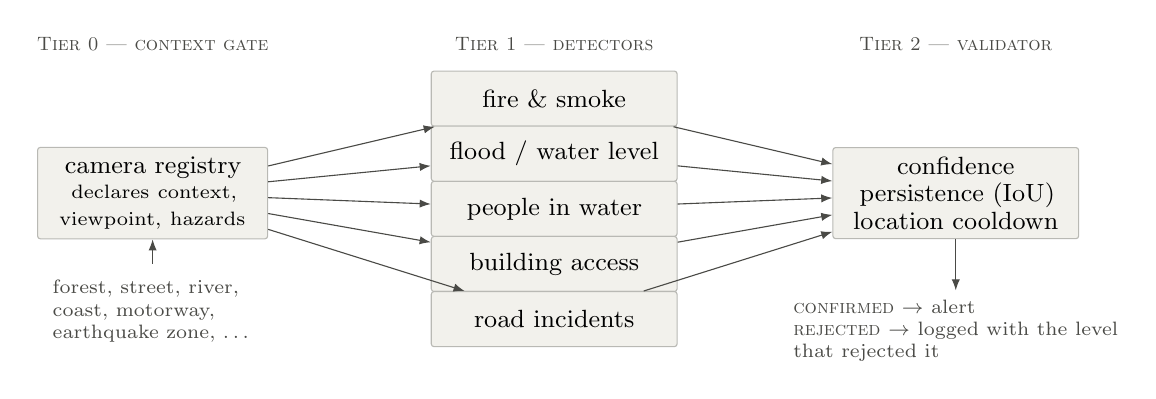
\begin{tikzpicture}[
  font=\small,
  box/.style={draw=rulegrey, fill=tierfill, rounded corners=1pt,
              minimum height=7mm, inner xsep=6pt, align=center},
  tier/.style={draw=none, font=\scriptsize\scshape, text=notegrey},
  arrow/.style={-{Latex[length=4pt]}, draw=notegrey},
]
\node[tier] (t0) at (0,3.3) {Tier 0 — context gate};
\node[tier] (t1) at (5.1,3.3) {Tier 1 — detectors};
\node[tier] (t2) at (10.2,3.3) {Tier 2 — validator};

\node[box, text width=25mm] (gate) at (0,1.4)
  {camera registry\\[1pt]\scriptsize declares context,\\[-1pt]\scriptsize
   viewpoint, hazards};

\node[box, text width=27mm] (d1) at (5.1,2.6) {fire \& smoke};
\node[box, text width=27mm] (d2) at (5.1,1.9) {flood / water level};
\node[box, text width=27mm] (d3) at (5.1,1.2) {people in water};
\node[box, text width=27mm] (d4) at (5.1,0.5) {building access};
\node[box, text width=27mm] (d5) at (5.1,-0.2) {road incidents};

\node[box, text width=27mm] (val) at (10.2,1.4)
  {confidence\\[-1pt] persistence (IoU)\\[-1pt] location cooldown};

\node[align=left, font=\scriptsize, text=notegrey] (out) at (10.2,-0.35)
  {\textsc{confirmed} $\rightarrow$ alert\\ \textsc{rejected} $\rightarrow$
   logged with the level\\ that rejected it};

\foreach \d in {d1,d2,d3,d4,d5} { \draw[arrow] (gate) -- (\d); }
\foreach \d in {d1,d2,d3,d4,d5} { \draw[arrow] (\d) -- (val); }
\draw[arrow] (val) -- (out);

\node[align=left, font=\scriptsize, text=notegrey] at (0,-0.1)
  {forest, street, river,\\ coast, motorway,\\ earthquake zone, \dots};
\draw[arrow] (0,0.5) -- (gate);
\end{tikzpicture}
\caption{The three tiers. The gate decides which detectors run for a given
camera; the detectors run independently and in parallel; one shared validator,
configured per hazard but never specialised per hazard, decides which
detections become events.}
\label{fig:architecture}
\end{figure}

\subsubsection{Tier 0 — the context gate}
\label{sec:gate}

Each camera is registered once with a declared context. The gate looks up
which detectors apply to that context and runs only those.

\begin{definition}[Gate]
\label{def:gate}
Let $\contexts$ be the set of camera contexts, $\hazards$ the set of hazards,
$\cameras$ the registered cameras, and
\[
  \viewpoints = \{\,\textsc{ground},\ \textsc{oblique},\ \textsc{nadir}\,\}
\]
the set of viewpoints. Each camera $c$ carries
a context $\chi(c) \in \contexts$ and a viewpoint $\nu(c) \in \viewpoints$.
The gate is a total map
\[
  G : \contexts \longrightarrow 2^{\hazards},
\]
and the detectors constructed for camera $c$ are
$\detectors(c) = \{\, d_h : h \in G(\chi(c)) \,\}$.
\end{definition}

The gate is declarative, not learned. We deliberately do not classify a frame
and route it: that introduces a misrouting failure mode on the critical path
and saves little. Every operational deployment we surveyed works this way — a
ridgeline wildfire camera never runs drowning detection. Published work on
cascaded gating in video pipelines~\citep{kang2017noscope,mao2018catdet}
reports 5--13$\times$ compute reduction at minimal accuracy cost; here the
gate is what makes five hazards affordable on one machine.

The gate's entire intelligence is \cref{tab:gate}, which is small enough to
audit at a glance. That is the trade being made: a wrong entry here is visible
in a YAML file and fixable by a human, whereas a misrouting classifier fails
silently.

\begin{table}[htbp]
\centering\small
\caption{The context-to-hazard map. The bias is toward including a hazard when
it is plausible, because a missed hazard is a life-safety failure whereas an
unnecessary detector costs only the compute the gate was saving. Where that
bias was resisted — motorway, which excludes flood — the reason is that
claiming a hazard outside a detector's measured envelope is worse than not
claiming it.}
\label{tab:gate}
\begin{tabularx}{\textwidth}{l l L}
\toprule
Context & Hazards enabled & Reasoning \\
\midrule
forest             & fire                              & PyroNear's stated envelope: fixed-mount wide-field, daylight \\
wildland interface & fire, road                        & Settlement meets vegetation, plus the roads people flee along \\
street             & flood, road, building access      & The DANA case: water rising, vehicles caught, people trapped \\
urban block        & flood, building access            & Dense built environment \\
river              & flood, drowning                   & Level and rate of rise, plus anyone swept in \\
coast              & drowning                          & Open water; the SeaDronesSee envelope \\
motorway           & road                              & Deliberately narrow: flood is plausible but outside the flood detector's calibrated envelope \\
earthquake zone    & building access                   & The DRespNeT envelope \\
UAV search         & building access, drowning         & Aerial search and rescue; both detectors are UAV-trained \\
\bottomrule
\end{tabularx}
\end{table}

\paragraph{The saving is reported, not assumed.}
For a registry of $\cameras$ cameras and $|\hazards|$ available hazards, the
gate's reduction in detector invocations per frame is
\begin{equation}
  \rho \;=\; 1 - \frac{\sum_{c \in \cameras} |G(\chi(c))|}
                      {|\cameras|\,|\hazards|}.
  \label{eq:gate-saving}
\end{equation}
On the demonstration registry shipped with the system (\GateCameras{}
cameras and $|\hazards| = \GateHazards$ available hazards), the gate requests
\GateGated{} detector invocations per frame instead of \GateUngated{}, so
$\rho = \GateReduction\,\%$, and only \GateModelsLoaded{} of the
\GateHazards{} detector types are ever constructed. The unrequested models are
never constructed at all, so the saving is in memory as well as compute: a
deployment of only ridgeline cameras loads one ONNX session, not five.

\subsubsection{Viewpoint envelopes}
\label{sec:viewpoint}

The gate also declares \emph{viewpoint}, because a detector's training
viewpoint is part of its operating envelope and nothing else in the system
captured it.

\begin{definition}[Admissibility]
\label{def:admissible}
Each detector $d$ declares an envelope $V(d) \subseteq \viewpoints$. A camera
$c$ may be paired with $d$ only if
\[
  \mathrm{adm}(c, d) \iff \nu(c) \in V(d),
\]
and $\mathrm{CameraPipeline}(c)$ raises unless
$\mathrm{adm}(c,d)$ holds for every $d \in \detectors(c)$.
\end{definition}

This was added after a measured failure, not as a precaution.

\begin{recorded}{A confident wrong number}
The flood segmenter is trained on ATLANTIS~\citep{erfani2022atlantis}, which
is ground-level and oblique photography of water bodies. Evaluated on
straight-down UAV imagery it reported up to $0.397$ water coverage on frames
whose actual water was a narrow canal, tinting large areas of mown grass as
water. It did not fail loudly. It returned a confident wrong number, which for
a life-safety component is the worst available failure. Viewpoint is therefore
declared on every camera and every detector, and the pipeline refuses the
pairing before any model is loaded — the same reasoning as the licence and
privacy guards: make the mistake impossible instead of documented. A test
fails the build if any detector stops declaring an envelope, so a sixth hazard
cannot be added without stating where it works.
\end{recorded}

\begin{recorded}{Failing loudly}
An unregistered camera raises instead of returning an empty hazard set.
Returning an empty set would turn a typo into a camera that watches for
nothing and reports success — the worst available failure mode for this
system. Enforced by \texttt{tests/test\_registry.py}.
\end{recorded}

\subsubsection{Tier 1 — specialist detectors}

Independent models running in parallel, rather than one shared-backbone
multi-task model. A unified model would require a single coherent label space
and jointly annotated data; these hazards come from separate datasets with
incompatible labels. It would also couple training, so that retraining fire
could silently degrade flood.

\subsubsection{Licensing architecture}
\label{sec:licensing}

VIGÍA ships under Apache-2.0. Several source models were fine-tuned using
Ultralytics tooling, which is licensed AGPL-3.0 — a licence whose terms would
extend to this entire project were the package imported at runtime.

The resolution is to run every model through ONNX Runtime and never import the
\texttt{ultralytics} package in the runtime path. PyroNear's own edge engine
does exactly this, which is how it remains Apache-2.0 while running a YOLO
architecture. Any \texttt{.pt}~$\rightarrow$~\texttt{.onnx} conversion is an
offline build step confined to \texttt{tools/}, executed in a separate virtual
environment.

This is enforced automatically, not by discipline:
\texttt{tools/check\_licence.py} parses every file under \texttt{vigia/} with
Python's AST module and fails the build if a forbidden package is imported. It
parses rather than greps, so a comment mentioning the package does not trip
it.

\subsubsection{Privacy by design}
\label{sec:privacy}

The EU AI Act's high-risk provisions~\citep{euaiact} took full effect in
August 2026. Annex III classifies biometric identification systems as
high-risk, and Article 5(1)(h) prohibits real-time remote biometric
identification in publicly accessible spaces for law enforcement, with narrow
exceptions.

VIGÍA identifies nobody, and this is structural, not configured.

\begin{table}[htbp]
\centering\small
\caption{Four privacy commitments and the mechanism that enforces each. A
commitment that lives only in a document is a configuration flag waiting to
happen.}
\label{tab:privacy}
\begin{tabularx}{\textwidth}{p{4.1cm} L}
\toprule
Commitment & How it is enforced \\
\midrule
No biometric code path &
\texttt{tools/check\_privacy.py} parses every file under \texttt{vigia/},
\texttt{tools/}, \texttt{scripts/} and \texttt{eval/} and fails on any import
of a face or re-identification library, any use of OpenCV's face APIs, or any
function or class whose name describes identity work. Unlike the licence
guard, \texttt{tools/} is not exempt: an offline script that built a face
index would breach the commitment just as surely. \\
\addlinespace
Only the event and one evidence frame leave &
The \texttt{Alert} type has no field for a clip and no writer for one. A test
asserts the absence, so adding one becomes a visible change to a documented
boundary rather than a quiet tweak. \\
\addlinespace
No raw video retention &
\texttt{RetentionPolicy} raises on construction if raw video storage is
requested. The rolling buffer is a fixed-length in-memory deque sized from the
camera's declared retention window, and no code path writes video to disk. \\
\addlinespace
Presence and location, never identity &
Person-shaped detections are blurred inside their own boxes before any
evidence frame is written, on a copy so the source frame is never mutated. The
box stays visible: an operator needs to know that someone is there and where,
never who. \\
\bottomrule
\end{tabularx}
\end{table}

The redaction list is keyed on detector class names, and a test fails if a
detector declares a person-depicting class that is not on it — so a sixth
hazard cannot introduce an unredacted person class by omission.

\begin{recorded}{Guards are tested against violations}
A guard that cannot fail is worthless. The privacy guard was run against
deliberately planted violations, which is how two gaps were found: class names
such as \texttt{PersonReidentifier} and \texttt{GaitSignatureExtractor}
initially escaped, because the patterns matched whole words containing
underscores. Matching now strips underscores before comparison. The same
reasoning applies to the ONNX parity check of \cref{sec:backends}.
\end{recorded}

\subsubsection{Runtime pipeline}
\label{sec:pipeline}

The three tiers are joined by \texttt{vigia/pipeline.py}: capture, gate,
detect in parallel, validate, emit. It decides none of those things itself —
the registry decides which detectors run, the validator decides what is an
alert, and the egress module decides what may leave. Keeping those three out
of the pipeline is what allows each to be tested and reported separately, and
it is why adding a sixth hazard touches none of this code.

Concurrency follows the pattern reported for a comparable
system~\citep{multitasksystem}: one
thread per active detector over bounded queues, with a single fusion stage.
The detectors are independent ONNX Runtime sessions, which release the GIL
during inference — where essentially all of the time goes — so they run
genuinely in parallel. Across cameras the detector objects are shared while
the validators are emphatically not: validator state is per camera per hazard,
and sharing it would let one camera's tracks confirm another camera's events.

The queues are bounded by design. An unbounded queue converts a detector that
cannot keep up into unbounded memory growth and ever-increasing latency, which
in a life-safety system means alerting about something that stopped being true
minutes ago. Bounded queues convert the same condition into dropped frames
that are counted and reported. How the backpressure resolves depends on the
source, and the distinction matters for the integrity of every figure here:

\begin{itemize}
  \item \textbf{Live sources never block.} A detector that falls behind costs
        frames, not latency, and stale frames are discarded in favour of the
        newest available.
  \item \textbf{File sources always block.} An evaluation replay or a curated
        demonstration clip must be deterministic; dropping frames would make a
        published measurement depend on how busy the machine happened to be.
\end{itemize}

\begin{recorded}{Found by measurement, not foresight}
With non-blocking dispatch on both source types, a 16-frame clip through a
\SI{193}{\milli\second} detector processed 3 frames and silently dropped 13. A
replay that quietly skips 80\,\% of its input would have produced plausible
and meaningless numbers.
\end{recorded}

On the reference machine a single ridgeline camera replaying a 40-frame
sequence through the fire detector sustains 8--14 frames per second end to end
at \SI{117}{\milli\second} median detector latency, processing every frame
with none dropped.

\subsection{Definitions and evaluation metrics}
\label{sec:metrics}

This section fixes the quantities the rest of the document reports. It exists
because several of the mistakes recorded here were mistakes of \emph{metric}
and not of model: a figure that was correct as computed and wrong as
interpreted. Stating the definitions precisely is what made those visible.

\subsubsection{Matching predictions to ground truth}

For two axis-aligned boxes $a, b$ the intersection over union is
\begin{equation}
  \iou(a,b) \;=\; \frac{|a \cap b|}{|a \cup b|} \;\in\; [0,1].
  \label{eq:iou}
\end{equation}

Given predictions $\hat{B} = \{\hat{b}_1, \dots, \hat{b}_m\}$ sorted by
descending confidence and ground truth $B = \{b_1, \dots, b_n\}$, each
prediction is matched greedily to the highest-$\iou$ unmatched ground-truth
box exceeding a threshold $\tau$. Writing $\mathrm{TP}$, $\mathrm{FP}$ and
$\mathrm{FN}$ for the resulting counts,
\begin{equation}
  \precision = \frac{\mathrm{TP}}{\mathrm{TP} + \mathrm{FP}}, \qquad
  \recall = \frac{\mathrm{TP}}{\mathrm{TP} + \mathrm{FN}}.
  \label{eq:pr}
\end{equation}

Throughout this document $\tau = 0.3$. That is looser than the $0.5$
convention, and the choice is deliberate: the operational question is whether
a person or a plume was \emph{found}, not whether its box was drawn tightly.
A stricter threshold answers a localisation question this system does not ask.

\subsubsection{Box-level and image-level evaluation}
\label{sec:twolevels}

\emph{Box-level} metrics use \cref{eq:pr} over instances. \emph{Image-level}
metrics reduce each image to a binary decision — did the detector fire at all
— and compute the same quantities over images. The image-level false-alarm
rate over a negative set $N$ (images containing no instance of the hazard) is
\begin{equation}
  \mathrm{FAR} \;=\; \frac{|\{\, i \in N : \hat{y}_i = 1 \,\}|}{|N|}.
  \label{eq:far}
\end{equation}

Both are reported everywhere, because either alone conceals a failure the
other exposes.

\begin{recorded}{The failure that image-level metrics hid}
The people-in-water detector's exported head has six logit slots for five
classes. A leading no-object slot was assumed, and every label shifted by one:
boats were reported as swimmers at $0.84$ confidence while real swimmers were
discarded. It nearly survived review because image-level precision still read
$0.83$ — boats and swimmers co-occur in the same frames, so an image with a
boat called ``swimmer'' is still an image containing a swimmer. Only
box-level $\iou$ matching exposed it, at a recall of $0.002$.
\end{recorded}

\subsubsection{Recall-weighted \texorpdfstring{$F$}{F} scores}

The harmonic family
\begin{equation}
  F_\beta \;=\; \frac{(1 + \beta^{2})\, \precision \recall}
                     {\beta^{2} \precision + \recall}
  \label{eq:fbeta}
\end{equation}
is reported at $\beta = 2$ as the headline, a convention borrowed from the
RipVIS benchmark~\citep{ripvis2025}. The justification is not stylistic. At
the symmetric point $\precision = \recall = p$,
\begin{equation}
  \frac{\partial F_\beta / \partial \recall}
       {\partial F_\beta / \partial \precision}
  \;=\; \beta^{2},
  \label{eq:fbeta-ratio}
\end{equation}
so $\beta = 2$ states explicitly that a point of recall is worth four points
of precision here. That is the correct trade for this system for an asymmetric
reason: the validator downstream can discard a false alarm, but nothing
downstream can recover a person who was never detected.

\subsubsection{Segmentation metrics and pooling}
\label{sec:pooling}

For binary masks the water $\iou$ on a single image is \cref{eq:iou} over
pixel sets. Over a corpus of $n$ images there are two ways to aggregate, and
they answer different questions:
\begin{align}
  \iou_{\text{pooled}} &= \frac{\sum_{i=1}^{n} |P_i \cap G_i|}
                               {\sum_{i=1}^{n} |P_i \cup G_i|},
  \label{eq:iou-pooled} \\[2pt]
  \iou_{\text{strat}}  &= \frac{\sum_{i \in S} |P_i \cap G_i|}
                               {\sum_{i \in S} |P_i \cup G_i|},
  \qquad S \subset \{1,\dots,n\}.
  \label{eq:iou-strat}
\end{align}

\Cref{eq:iou-pooled} weights every image by the size of its union, so a corpus
dominated by easy cases is dominated by easy cases in the score. When the
subset $S$ that the model exists to handle is a small minority, the pooled
figure flatters it, and the more severe the case the smaller its influence.

This is not hypothetical. FloodNet's~\citep{rahnemoonfar2021floodnet} labelled
release contains \AerialLabelled{} pairs of which only \AerialFlooded{} are
flooded — \AerialFloodedShare\,\% of the corpus. The aerial flood segmenter
scores $\iou_{\text{pooled}} = \AerialOverallIoU$ but
$\iou_{\text{strat}} = \AerialFloodedIoU$ on the flooded subset. Model
selection in this project uses the stratified figure, and \cref{sec:flood}
publishes it as the headline with the pooled one beside it, clearly labelled.
Selecting on the pooled figure would have chosen a model that is better at
recognising dry ground.

\subsubsection{Interval estimation}
\label{sec:intervals}

Half of this project's figures rest on small samples: \BuildingTestImages{}
held-out images for building access, \FireNarrowNegatives{} negatives in the
first fire baseline. A bare point estimate from such a sample invites a reader
to believe it to three decimal places, so every proportion in this document
whose denominator is known is reported with a 95\,\% \emph{Wilson score}
interval~\citep{wilson1927probable}. For $k$ successes in $n$ trials with
$\hat{p} = k/n$ and $z = 1.96$,
\begin{equation}
  \mathrm{CI}_{95} \;=\;
  \frac{\hat{p} + \dfrac{z^{2}}{2n}}{1 + \dfrac{z^{2}}{n}}
  \;\pm\;
  \frac{z\sqrt{\dfrac{\hat{p}(1-\hat{p})}{n} + \dfrac{z^{2}}{4n^{2}}}}
       {1 + \dfrac{z^{2}}{n}}.
  \label{eq:wilson}
\end{equation}

Wilson over the textbook normal approximation
$\hat{p} \pm z\sqrt{\hat{p}(1-\hat{p})/n}$, for a reason this project's data
makes concrete instead of academic~\citep{brown2001interval}. At
$\hat{p} = 1$ the normal interval collapses to a point: building access
detects a person in $12$ of $12$ positive held-out images, and the normal
interval reports $[1.000, 1.000]$ — perfect certainty inferred from twelve
observations. \Cref{eq:wilson}, derived by inverting the score test rather
than by assuming normality of the estimate, gives
\BuildingImageRecallCI. That interval is the honest statement, and it is what
\cref{sec:building} reports.

\Cref{tab:intervals} collects the cases where the interval changes how a
figure should be read.

\begin{table}[htbp]
\centering\small
\caption{Point estimates with the 95\,\% Wilson interval their sample size
supports. The last column is the reading the interval permits, which in three
of these rows is materially weaker than the point estimate alone suggests.
Computed from the measurement files.}
\label{tab:intervals}
\begin{tabularx}{\textwidth}{l S[table-format=1.4] c L}
\toprule
Quantity & {Estimate} & 95\,\% interval & What it supports \\
\midrule
Fire image-level FAR, \FireNegatives{} negatives
  & \FireImageFAR & \FireImageFARCI
  & Precise enough to quote. The motivating claim is safe. \\
Fire image-level FAR, \FireNarrowNegatives{} negatives
  & \FireNarrowFAR & \FireNarrowFARCI
  & Consistent with anything from two-thirds to nearly all. Withdrawn. \\
Swimmer box recall, \SwimmerInstances{} instances
  & \SwimmerBoxRecall & \SwimmerBoxRecallCI
  & Tight. The strongest evidence in the project. \\
Civilian box recall, \BuildingCivilians{} instances
  & \BuildingCivilianRecall & \BuildingCivilianRecallCI
  & Solid at instance level, from \BuildingTestImages{} images. \\
Building image-level recall, 12 images
  & \BuildingImageRecall & \BuildingImageRecallCI
  & Cannot exclude one image in four being missed. \\
Building image-level FAR, 12 negatives
  & \BuildingImageFAR & \BuildingImageFARCI
  & Almost uninformative. Reported for completeness only. \\
Scene router accuracy, \RouterHeldOut{} images
  & \RouterAccuracy & \RouterAccuracyCI
  & Tight, but see \cref{sec:routing} on task difficulty. \\
\bottomrule
\end{tabularx}
\end{table}

\subsubsection{Class merging}

Two detectors emit more classes than VIGÍA consumes. Merging is a partial
surjection
\begin{equation}
  \mu : \mathcal{K}_{\text{model}} \longrightarrow
        \mathcal{K}_{\text{system}} \cup \{\bot\},
  \label{eq:merge}
\end{equation}
where $\bot$ discards a class. For building access $|\mathcal{K}_{\text{model}}| = 28$
and $|\mathcal{K}_{\text{system}}| = 5$; for people in water, five model classes
reduce to one consumed class. Crucially, $\mu$ is applied at the detector
boundary and only a designated subset
$\mathcal{A} \subseteq \mathcal{K}_{\text{system}}$ — the \emph{alarm} classes
— reaches the validator. Everything else is operator context. A rescue team on
site is the expected state at an incident already being handled, and a boat is
not an emergency; routing either to the validator would alarm on every rescue
worker and every vessel in frame.

\section{Detectors}
\label{sec:detectors}

One subsection per hazard. Each names the people whose work it uses, states
what we changed, and reports only figures we measured ourselves; figures
published by the original authors are listed separately and attributed.

Five hazards are integrated. Four are disaster hazards and carry the system's
purpose; the fifth, road incidents, is retained explicitly as a generality
experiment for the validator rather than as a headline capability — a car
accident is an emergency, not a disaster. Its value is that it has completely
different physics and timescales from wildfire, so a validator that works on
both is demonstrably not tuned to one phenomenon.

\subsection{Fire and smoke}
\label{sec:fire}

\begin{description}[leftmargin=7.4em,labelwidth=7.0em,style=sameline,font=\normalfont\itshape]
  \item[Model] \texttt{yolo11s\_sensitive-detector}, Apache-2.0.
  \item[Authors] The PyroNear association, a French open-source non-profit, in
    collaboration with the French Fire and Rescue Services
    (SDIS)~\citep{pyronear2025}.
  \item[Deployment] 15 lookout towers, 51 cameras across France, Spain and
    Chile, running on Raspberry Pi hardware.
  \item[Envelope] Fixed-mount wide-field outdoor cameras viewing a landscape
    horizon, in daylight. Not validated for indoor fire, close-range flame or
    night operation.
\end{description}

It is a deliberately \emph{sensitive} detector: the authors recommend a low
confidence floor ($0.20$) and a very low NMS $\iou$ ($0.01$), trading
precision for recall on the assumption that a downstream filter exists. That
design choice is precisely why it is the right baseline for this project — the
filter it assumes is what we built.

We run the published ONNX export unmodified. The model is downloaded from its
original distributor at setup time and is never redistributed here. We
relabelled its single class from \texttt{item} to \texttt{smoke}, and wrote
our own letterbox preprocessing and YOLO decoding with NumPy non-maximum
suppression, so the runtime has no dependency on the AGPL-licensed package
(\cref{sec:licensing}).

\begin{table}[htbp]
\centering\small
\caption{Fire detector, single-frame and with no temporal validation — this is
the baseline the validator must improve on, not a headline result.
\texttt{pyro-sdis}~\citep{pyrosdis} validation split, \FireImages{} rows
(\FirePositives{} positive, \FireNegatives{} negative, 21 cameras), confidence
$0.20$, $\tau = 0.3$. \measured{} — \texttt{eval/run\_image\_eval.py}.}
\label{tab:fire}
\begin{tabular}{l S[table-format=1.3] l}
\toprule
Metric & {Value} & Note \\
\midrule
Box precision              & \FireBoxPrecision & \\
Box recall                 & \FireBoxRecall    & \\
Box $F_2$                  & \FireBoxFTwo      & recall-weighted, \cref{eq:fbeta} \\
Image-level recall         & \FireImageRecall  & \\
Image-level FAR            & \FireImageFAR     & 95\,\% CI \FireImageFARCI \\
Median latency, ms & \FireLatency & M4 Pro, CPU provider \\
\bottomrule
\end{tabular}
\end{table}

The authors publish no precision, recall or mAP for this checkpoint, so
\cref{tab:fire} has no \reported{} column: there is nothing to compare
against, and inventing one would be worse than the gap.

\begin{recorded}{A caveat that earned its keep}
The most quoted figure in this project — that the published fire detector
alarms on frames containing no smoke — was first measured on
\FireNarrowNegatives{} negative frames and carried the standing note
``indicative, not precise; widen before publishing''. Widening it to
\FireNegatives{} negatives from 21 cameras, a twenty-five-fold increase, moved
the false-alarm rate from \FireNarrowFAR{} to \FireImageFAR{} and box
precision from \FireNarrowBoxPrecision{} to \FireBoxPrecision. Recall barely
moved (\FireNarrowBoxRecall{} to \FireBoxRecall), which is the reassuring
half: the detector finds what it finds, and it was the small sample that had
flattered it on false alarms. The motivating claim is untouched — a detector
alarming on 71\,\% of clear frames is unusable without a filter — but the
specific number was overstated by sixteen percentage points and every
quotation of it was corrected. \Cref{tab:intervals} shows why the original was
never quotable: its interval was \FireNarrowFARCI.
\end{recorded}

\begin{figure}[htbp]
\centering
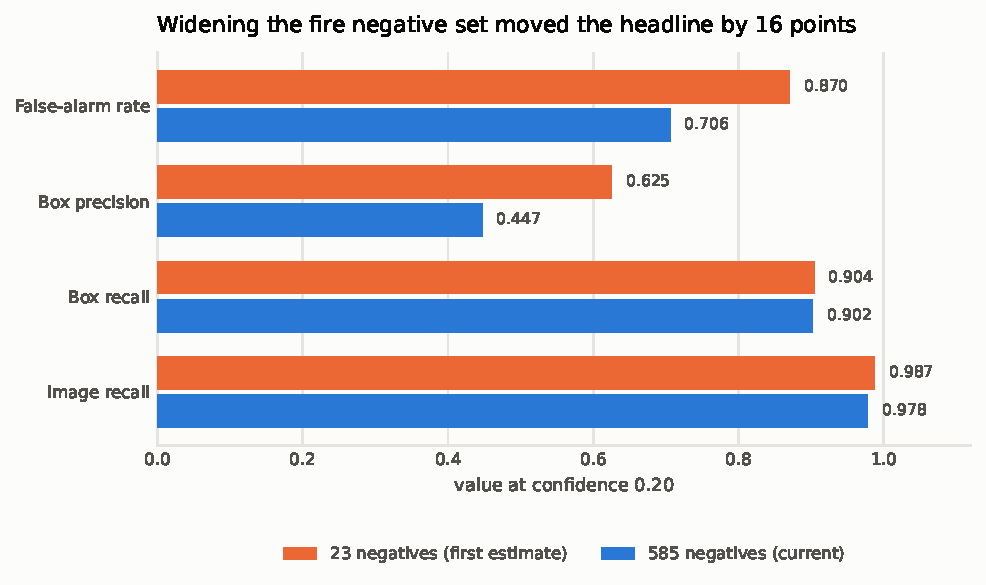
\includegraphics[width=0.85\textwidth]{fire_negative_widening.pdf}
\caption{The same detector at the same threshold, measured against
\FireNarrowNegatives{} negatives and then against \FireNegatives{}. Recall
barely moved; precision and the false-alarm rate both fell. This is what a
small sample flattering a detector looks like.}
\label{fig:widening}
\end{figure}

\subsection{Flood and water level}
\label{sec:flood}

The keystone hazard, and the one directly connected to the DANA. Two
capabilities: segmenting the water region, and estimating water level against
a fixed per-camera reference line (\cref{sec:flood-trend}).

\begin{description}[leftmargin=7.4em,labelwidth=7.0em,style=sameline,font=\normalfont\itshape]
  \item[Architecture] DeepLabV3~\citep{chen2017rethinking} with a
    MobileNetV3-Large backbone~\citep{howard2019searching}, from torchvision
    (BSD-3-Clause).
  \item[Training data] ATLANTIS~\citep{erfani2022atlantis} — 5{,}195
    pixel-annotated waterbody images, 56 classes.
  \item[Trained by] Us. This is the only ground-level detector in VIGÍA that
    we trained ourselves.
  \item[Envelope] Water region segmentation in outdoor scenes, ground and
    oblique viewpoints. The per-camera reference line is optional: without
    calibration the uncalibrated area signal still yields a trend, so a camera
    is useful the moment it is connected.
\end{description}

The architecture was chosen for licensing as much as performance: torchvision
is BSD-3-Clause, making this the only detector in the system entirely free of
AGPL. ATLANTIS's 56 classes were collapsed to binary water by
\cref{eq:merge} — VIGÍA does not need to know whether it is looking at a canal
or a river, only where the water is and whether it is rising. Seventeen
liquid-water labels count as water; water-associated \emph{structures} (dam,
levee, pier, culvert, breakwater) are excluded because they are not water, as
are glaciers and snow, which are not liquid, and mangrove, which is vegetation
standing in water whose extent does not track a level. The class mapping was
derived empirically by cross-referencing the dominant mask value in each label
folder against the published label list, not assumed.

\begin{table}[htbp]
\centering\small
\caption{Flood segmenter on the ATLANTIS test split, \FloodTestImages{}
images, held out and never seen during training or validation. No third-party
baseline is quoted because the dataset authors' own network reports over all
56 classes rather than binary water, so its figures are not comparable.
\measured{} — \texttt{eval/run\_flood\_eval.py}.}
\label{tab:flood}
\begin{tabular}{l S[table-format=1.4] l}
\toprule
Metric & {Value} & Note \\
\midrule
Water $\iou$    & \FloodWaterIoU      & pooled, \cref{eq:iou-pooled} \\
Precision       & \FloodPrecision     & \\
Recall          & \FloodRecall        & \\
$F_1$           & \FloodFOne          & \\
Pixel accuracy  & \FloodPixelAccuracy & \\
Median latency, ms & \FloodLatency & M4 Pro, CPU provider \\
\bottomrule
\end{tabular}
\end{table}

\begin{recorded}{A deployment hazard in the export}
PyTorch's ONNX exporter splits weights into a separate \texttt{.onnx.data}
sidecar. Copying only the \texttt{.onnx} yields a graph that loads
successfully and then produces garbage. Our export folds any sidecar back into
the single file and verifies argmax parity against the source PyTorch model,
failing below 99.9\,\% agreement.
\end{recorded}

\subsubsection{The aerial variant}

A UAV camera declaring a \textsc{nadir} viewpoint was previously refused by
\cref{def:admissible}, because the ATLANTIS model's envelope excludes it. A
second segmenter was therefore trained on FloodNet Track
1~\citep{rahnemoonfar2021floodnet} (CDLA-Permissive-1.0) and the pipeline
routes by viewpoint.

Its evidence class is weaker than everything else in this document and is
labelled as such: FloodNet withheld its validation and test masks for the
competition, so no independent labelled split exists in the release. The
figures below come from a stratified split carved out of the
\AerialLabelled{} labelled training pairs and \emph{seen by model selection} —
training-time validation, not held-out evaluation.

\begin{table}[htbp]
\centering\small
\caption{Aerial flood segmenter. Two $\iou$ figures are reported because
\cref{sec:pooling} requires it: only \AerialFlooded{} of \AerialLabelled{}
labelled images are flooded, so the pooled figure is carried by dry scenes.
Model selection used the stratified figure. \textsc{validation-measured}, not
held out — \texttt{scripts/train\_flood\_aerial.py}.}
\label{tab:flood-aerial}
\begin{tabular}{l S[table-format=1.4] l}
\toprule
Metric & {Value} & Note \\
\midrule
Water $\iou$, flooded subset & \AerialFloodedIoU   & \cref{eq:iou-strat}; the honest figure \\
Water $\iou$, pooled         & \AerialOverallIoU   & \cref{eq:iou-pooled}; flattered by dry scenes \\
Pixel accuracy               & \AerialPixelAccuracy & \\
Best epoch                   & \AerialBestEpoch    & selected on the flooded subset \\
\bottomrule
\end{tabular}
\end{table}

\begin{figure}[htbp]
\centering
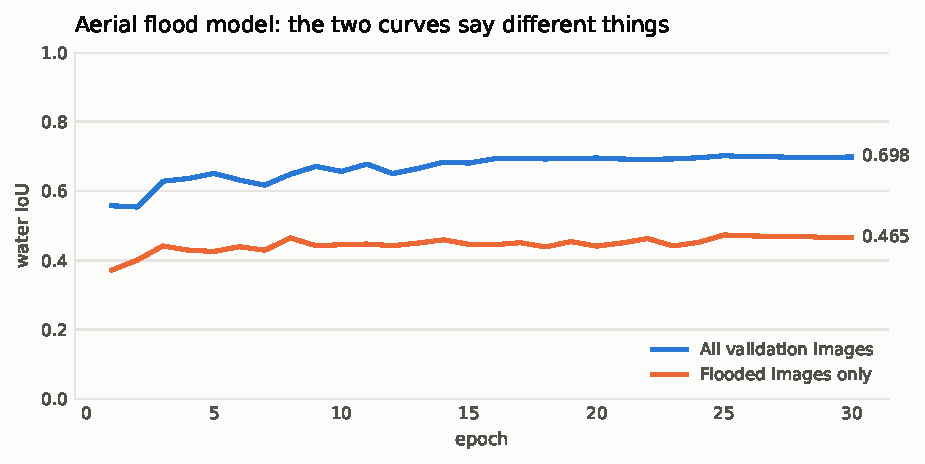
\includegraphics[width=0.85\textwidth]{aerial_flood_training.pdf}
\caption{Training the aerial flood segmenter. The two curves are reported
separately because only \AerialFlooded{} of \AerialLabelled{} labelled images
are flooded; a single pooled $\iou$ would be carried by dry scenes and would
flatter the model on the one case it exists to handle.}
\label{fig:aerial}
\end{figure}

\subsection{People in water}
\label{sec:piw}

\begin{description}[leftmargin=7.4em,labelwidth=7.0em,style=sameline,font=\normalfont\itshape]
  \item[Model] RF-DETR Small fine-tuned on SeaDronesSee~\citep{rfdetrseadronessee},
    Apache-2.0.
  \item[Dataset] SeaDronesSee~\citep{varga2022seadronessee}, CC0 1.0 — the
    least restrictive licence in the project, so the credit here is given by
    choice rather than obligation.
  \item[Why RF-DETR] The same author published YOLO11n and YOLO11x checkpoints
    for this dataset under AGPL-3.0. RF-DETR was chosen specifically because
    it is Apache-2.0 and keeps this detector outside the AGPL perimeter.
  \item[Envelope] Elevated and aerial views of open water,
    \SIrange{5}{260}{\metre} altitude. Not validated for pool settings, surf
    zones or extreme crowd density.
\end{description}

Only the \texttt{swimmer} class reaches the validator. A boat is context, not
an emergency. RF-DETR emits a fixed set of object queries with no duplicate
boxes, so unlike the YOLO detectors it requires no non-maximum suppression.

\begin{table}[htbp]
\centering\small
\caption{People-in-water detector, SeaDronesSee validation split,
\SwimmerImages{} images (\SwimmerPositiveImages{} with swimmers),
\SwimmerInstances{} ground-truth swimmer instances, confidence $0.30$.
\measured{} — \texttt{eval/run\_person\_in\_water\_eval.py}.}
\label{tab:piw}
\begin{tabular}{l S[table-format=1.4] l}
\toprule
Metric & {Value} & Note \\
\midrule
Swimmer box precision & \SwimmerPrecision & \\
Swimmer box recall    & \SwimmerRecall    & 95\,\% CI \SwimmerBoxRecallCI \\
Swimmer box $F_1$     & \SwimmerFOne      & \\
Image-level FAR       & \SwimmerImageFAR  & 95\,\% CI \SwimmerImageFARCI \\
Median latency, ms & \SwimmerLatency & M4 Pro, CPU provider \\
\bottomrule
\end{tabular}
\end{table}

We do not quote the author's headline mAP@50 of \SwimmerAuthorMAP{}
(\reported{}): it is across five classes and carried by boats, and the swimmer
class — the only one VIGÍA cares about — is their second weakest at
\SwimmerAuthorAP{} (\reported{}). Our \SwimmerFOne{} and their
\SwimmerAuthorAP{} are not in conflict. Average precision over strict $\iou$
thresholds punishes imprecise boxes on tiny objects, while our
$\tau = 0.3$ operating point asks the operationally relevant question, which
is whether the person was found at all.

\begin{figure}[htbp]
\centering
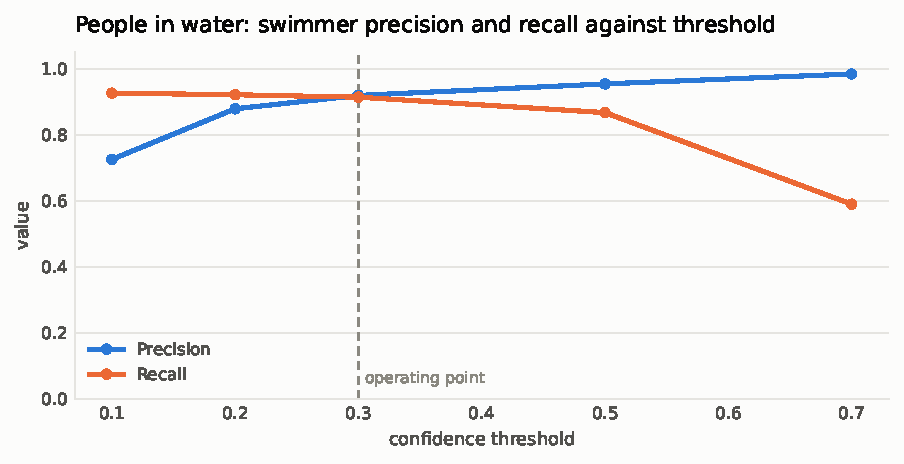
\includegraphics[width=0.85\textwidth]{confidence_sweep.pdf}
\caption{Swimmer precision and recall against the confidence threshold. The
operating point is chosen where recall is still high, because the validator
can discard a false alarm but nothing downstream can recover a person never
detected — the same asymmetry that motivates $\beta = 2$ in
\cref{eq:fbeta-ratio}.}
\label{fig:sweep}
\end{figure}

\subsection{Trapped people and building access}
\label{sec:building}

\begin{description}[leftmargin=7.4em,labelwidth=7.0em,style=sameline,font=\normalfont\itshape]
  \item[Model] YOLOv8-DRN, trained and published by the DRespNeT
    authors~\citep{sirma2025drespnet}, CC BY 4.0 — attribution is legally
    required here, unlike SeaDronesSee where it is given by choice.
  \item[Dataset] DRespNeT: UAV imagery of the 2023 Türkiye earthquakes,
    650 train / 50 valid / 25 test.
  \item[Envelope] Downward and oblique UAV views of earthquake-damaged urban
    blocks. Not validated for street-level views, interior imagery or night.
    Trained on 650 images, so generalisation to other disaster types and other
    cities is unproven rather than assumed.
\end{description}

The model predicts 28 classes; \cref{eq:merge} reduces them to five at the
detector boundary, and only \texttt{civilian} reaches the validator. The model
is an instance segmenter, so its output carries 32 mask coefficients after the
class scores; these are trimmed at postprocess, because without that the
decoder reads 60 classes and takes an argmax over mask prototypes.

\begin{table}[htbp]
\centering\small
\caption{Building-access detector on the held-out test split,
\BuildingTestImages{} images, \BuildingCivilians{} ground-truth civilian
instances, confidence $0.30$. The image-level rows are computed over twelve
positive and twelve negative images; their intervals are given because the
point estimates alone would badly overstate what \BuildingTestImages{} images
can establish. \measured{} — \texttt{eval/run\_building\_access\_eval.py}.}
\label{tab:building}
\begin{tabular}{l S[table-format=1.3] l}
\toprule
Metric & {Value} & Note \\
\midrule
Civilian box precision & \BuildingBoxPrecision & \\
Civilian box recall    & \BuildingBoxRecall    & 95\,\% CI \BuildingCivilianRecallCI \\
Civilian box $F_1$     & \BuildingBoxFOne      & \\
Image-level recall     & \BuildingImageRecall  & 95\,\% CI \BuildingImageRecallCI \\
Image-level FAR        & \BuildingImageFAR     & 95\,\% CI \BuildingImageFARCI \\
Rescue team $F_1$      & \BuildingRescueFOne   & operator context, not an alarm \\
Accessible entry $F_1$ & \BuildingEntryOpenFOne & operator context \\
Blocked entry $F_1$    & \BuildingEntryBlockedFOne & operator context \\
Collapsed building $F_1$ & \BuildingCollapsedFOne & operator context \\
Median latency, ms & \BuildingLatency & M4 Pro, CPU provider \\
\bottomrule
\end{tabular}
\end{table}

The authors report 92.7\,\% mAP@50 at 27\,FPS across all 28 classes
(\reported{}). That is not comparable to \cref{tab:building}: they report over
28 classes, we merge to five and measure one.

\begin{recorded}{An architectural preference abandoned on evidence}
VIGÍA first trained its own torchvision Faster R-CNN on the same 650 images,
specifically because torchvision is BSD-3-Clause and would have kept this
detector clear of the AGPL perimeter altogether. On the identical held-out
split with the identical metric it reached civilian box recall of $0.141$ — it
missed roughly six of every seven people it should have boxed, and was by a
wide margin the weakest component in the system. The authors' own weights
reach \BuildingBoxRecall. The test/valid gap also inverted: our model scored
$0.462$ on valid against $0.141$ on test, a collapse showing it had not
generalised, where the published weights score $0.815$ against
\BuildingBoxFOne. Keeping a six-times-worse detector to preserve an
architectural preference would have been a choice against the people this
detector exists to find. The AGPL exposure is contained the same way as fire:
ONNX conversion in an isolated build environment, no weights redistributed,
enforced by \texttt{tools/check\_licence.py}.
\end{recorded}

\begin{figure}[htbp]
\centering
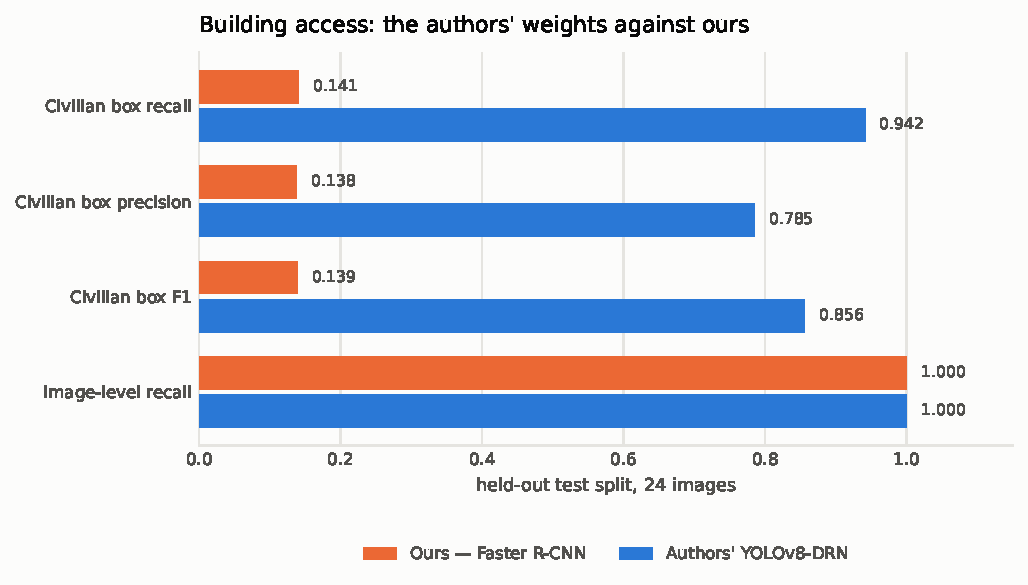
\includegraphics[width=0.85\textwidth]{building_access_models.pdf}
\caption{The two models on the identical held-out split with the identical
metric. Image-level recall is \BuildingImageRecall{} for both, which is
exactly why image-level metrics alone are not enough (\cref{sec:twolevels}):
they hide a six-fold difference in whether the person was actually located.}
\label{fig:building-models}
\end{figure}

\begin{figure}[htbp]
\centering
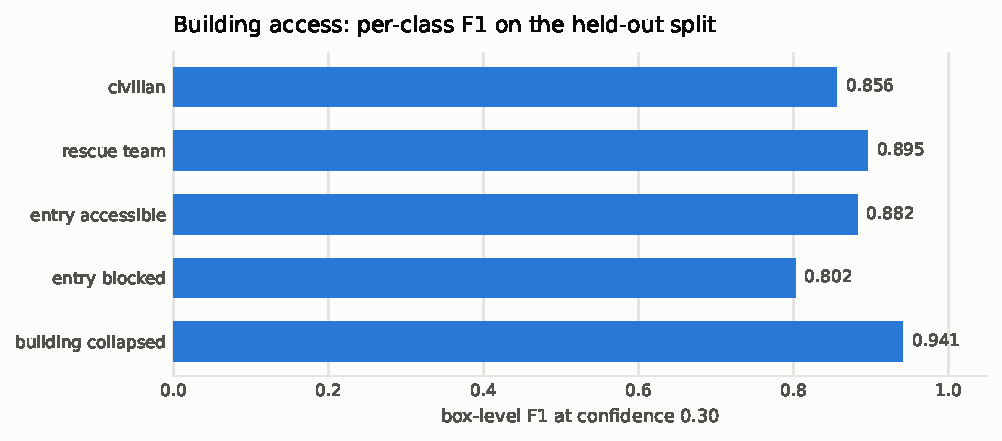
\includegraphics[width=0.85\textwidth]{building_access_per_class.pdf}
\caption{Per-class $F_1$ on the held-out split at confidence $0.30$. Only
\texttt{civilian} reaches the validator; the rest are operator context.}
\label{fig:building-classes}
\end{figure}

\subsection{Road incidents}
\label{sec:traffic}

Included to test whether the validator transfers to a hazard with entirely
different physics. The model~\citep{enostraffic} is MIT-licensed and detects
accidents and vehicles in roadside and dashcam imagery; only the
\texttt{accident} class reaches the validator, since passing \texttt{vehicle}
through would make every car on the road an alert.

Its status is \emph{not measured}. It is integrated and running behind the
validator, and it supplied the second hazard in \cref{tab:transfer}, but that
experiment measures the \emph{validator}, not this detector: no precision or
recall for the accident class against held-out labels has been run. The
available footage is a dashcam compilation that is predominantly accident
footage and therefore cannot support a false-positive rate. The authors report
mAP@50 of $0.826$ and accident-class recall of $0.855$ (\reported{}); we do
not adopt those as ours.

\begin{recorded}{A checkpoint choice recorded rather than silently made}
The author's own inference script uses the \texttt{epoch14} checkpoint. On
their four published test images, \texttt{epoch61} returns exactly one
accident per image at confidence $0.58$--$0.70$, whereas \texttt{epoch14}
returns three detections on one image. We use \texttt{epoch61} and record the
reason here rather than leaving a future reader to wonder why the two
disagree.
\end{recorded}

\section{The anticipatory flood signal}
\label{sec:flood-trend}

Flood is the only hazard whose temporal logic does not rest solely on the
validator. A water level has a trend, and the trend is the alert: knowing that
a street is flooded is useful, but knowing that it is filling, and how fast,
is what buys evacuation time.

\paragraph{Not a novel contribution, and read this before describing it as
one.} \Citet{choi2026pagehinkley} target the same gap on the same
infrastructure — anticipatory urban flood warning from existing CCTV, using
Page--Hinkley change detection with short-term trend analysis producing an
estimated time-to-threshold. That is the same capability, published
independently. VIGÍA therefore implements \emph{both} mechanisms and measures
them against each other on identical inputs, rather than claiming either. What
is ours is the multi-hazard pipeline they sit inside.

\subsection{Two signals}

Segmenting water yields a mask $W_t \subseteq \Omega$ over the frame domain
$\Omega$. Two scalars are derived, deliberately:
\begin{align}
  a_t &= \frac{|W_t|}{|\Omega|}
     &&\text{area fraction — needs no calibration}
     \label{eq:area}\\
  \ell_t &= \frac{1}{K}\max\{\, k : \textstyle\sum_{j=k-4}^{k}
              \mathbb{1}[\, p_j \in W_t \,] > 0 \,\}
     &&\text{level along a reference line}
     \label{eq:level}
\end{align}
where $p_1, \dots, p_K$ are $K = 200$ points sampled from the bottom of a
per-camera reference line upward. \Cref{eq:level} walks up from the bottom and
stops at the first sustained dry stretch rather than taking the highest water
pixel anywhere on the line; a reflection or a puddle further up would
otherwise read as a far higher level than reality. The five-sample tolerance
is 2.5\,\% of the line, which absorbs segmentation speckle without jumping
gaps.

The area signal works on any camera the moment it is connected; the level
signal needs a one-off human calibration but is physically meaningful and
comparable between cameras. Choosing the reference line is deliberately not
automated: a wrong automatic choice would silently corrupt every reading from
that camera.

\subsection{Windowed least squares}

Rate of rise is fitted, not differenced. Frame-to-frame differencing of
a noisy segmentation mask produces a rate estimate dominated by segmentation
jitter; an ordinary least-squares slope over a window is stable enough to
threshold on. Over the readings in a trailing window $\mathcal{W}$,
\begin{equation}
  \hat{\beta} = \frac{\sum_{i \in \mathcal{W}} (t_i - \bar{t})(y_i - \bar{y})}
                     {\sum_{i \in \mathcal{W}} (t_i - \bar{t})^{2}},
  \qquad
  R^{2} = 1 - \frac{\sum_i (y_i - \hat{y}_i)^{2}}
                   {\sum_i (y_i - \bar{y})^{2}}.
  \label{eq:ols}
\end{equation}
A trend is declared only when $|\mathcal{W}| \ge 4$ and $R^{2} \ge 0.5$: a
poor fit usually means the segmentation is unstable rather than that the water
is doing something complicated, so the system declines to call it. Where a
calibrated level exists it is preferred over area for the trend decision,
because area fraction moves with camera perspective and level does not. The
operational output is the extrapolation
\begin{equation}
  t_{\text{threshold}} = \frac{\ell^{*} - \ell_t}{\hat{\beta}},
  \qquad \hat{\beta} > 0,
  \label{eq:tttp}
\end{equation}
which is the number an operator actually wants: not ``the street is flooding''
but ``this underpass is impassable in eleven minutes''.

\begin{recorded}{A bug only real data could find}
With a fixed \SI{300}{\second} window, \cref{eq:ols} never fired at all on a
creek camera sampled every fifteen minutes — it reported \textsc{unknown} for
seven hours while the water rose by 10\,\% of the frame — because the window
could never contain two frames. Every synthetic test passed throughout. A time
window is the wrong abstraction when the sampling rate is a property of the
deployment, so the window is now adaptive: it admits at least four sampling
intervals, measured from the observed median gap. Page--Hinkley, being
sample-based, not time-based, was unaffected.
\end{recorded}

\subsection{Page--Hinkley change detection}
\label{sec:ph}

The Page--Hinkley test~\citep{page1954continuous,hinkley1971inference} is a
classical sequential change-point detector. For observations $x_1, x_2, \dots$
with running mean $\bar{x}_i$, tolerated drift $\delta$ and threshold
$\lambda$:
\begin{align}
  m_t &= \sum_{i=1}^{t} \bigl( x_i - \bar{x}_i - \delta \bigr),
  \label{eq:ph-cum}\\
  M_t &= \min_{1 \le i \le t} m_i,
  \label{eq:ph-min}\\
  \mathrm{PH}_t &= m_t - M_t,
  \label{eq:ph-stat}
\end{align}
with an alarm at the first $t \ge t_{\min}$ for which
$\mathrm{PH}_t > \lambda$. Its character differs from \cref{eq:ols}: it
responds quickly to the \emph{onset} of a change, whereas the fit estimates
the \emph{rate} of an ongoing one more stably. They are complementary rather
than competing, which is why both are available.

\subsection{Calibration matters more than the algorithm}
\label{sec:ph-calibration}

On a signal that is not changing, \cref{eq:ph-cum} is a random walk with step
standard deviation $\sigma$ and drift $-\delta$ per sample, and
\cref{eq:ph-stat} is that walk's drawdown below its own running minimum. A
threshold small relative to the noise will therefore be crossed eventually by
noise alone. For Brownian motion with negative drift the all-time maximum
drawdown is exponentially distributed, giving
\begin{equation}
  \Pr[\text{false alarm}] \;\approx\;
  \exp\!\left( -\,\frac{2\,\delta\,\lambda}{\sigma^{2}} \right),
  \label{eq:ph-far}
\end{equation}
and, inverting, a design rule for a camera nobody has calibrated:
\begin{equation}
  \lambda \;\gtrsim\; \frac{\sigma^{2}}{2\delta}\,\ln\frac{1}{\alpha}
  \label{eq:ph-design}
\end{equation}
for a target false-alarm probability $\alpha$.

Our first defaults, $\delta = 0.002$ and $\lambda = 0.02$, looked reasonable
and produced a 92\,\% false-alarm rate on \emph{stable} water with realistic
segmentation noise. \Cref{tab:ph} places the measured grid beside
\cref{eq:ph-far}.

\begin{table}[htbp]
\centering\small
\caption{Page--Hinkley false-alarm rate on stable water, measured over 200
trials of 40 samples, against the drawdown model of \cref{eq:ph-far}. All
values are percentages. The model consistently \emph{under}-predicts — by
roughly a factor of two in the interesting region — because it assumes the
infinite-time limit and treats the running-mean subtraction as exact. It
nevertheless reproduces the ordering across every row and column and locates
the usable/unusable boundary correctly, so \cref{eq:ph-design} is a sound
floor for a new camera and not a substitute for measuring it. Generated by
\texttt{docs/build\_paper.py} from
\texttt{eval/results/page\_hinkley\_calibration.json}.}
\label{tab:ph}
\input{generated/page_hinkley}
\end{table}

The chosen default, $\delta = 0.005$ and $\lambda = 0.10$, trades a little
latency for zero false alarms at typical segmentation noise: detection latency
for a genuine rise is 11, 7 and 4 samples at 0.5\,\%, 1\,\% and 3\,\% per
frame respectively. A camera with noisier segmentation needs a higher
threshold, and \cref{eq:ph-design} says roughly how much higher — but it
should be measured per camera, not assumed.

\subsection{Compared on real cameras}

Both mechanisms were run on identical inputs from LSU creek camera sequences
in the V-FloodNet dataset~\citep{liang2022vfloodnet}: real fixed cameras, real
water, real segmentation noise. The two win on different sampling regimes —
the windowed fit is faster on densely sampled cameras, Page--Hinkley on
sparsely sampled ones, because it counts samples rather than seconds. Neither
is claimed as ours, and the comparison is reported; no winner is
declared.

\subsection{Ground truth the other footage does not have}
\label{sec:gage}

USGS cameras~\citep{usgshivis} sit on instrumented gauges, so every frame
arrives with a measured water level beside it — which no other footage in this
project provides. Over the 50 frames of a real flood event (Walnut Creek at
Raleigh, 8 August 2024, gauge rising to \SI{9.00}{\foot} and receding to
\SI{4.25}{\foot}), segmented water coverage correlates with measured gauge
height at $r = +0.50$.

That is a real but moderate relationship, and it is reported because it
\emph{qualifies} the trend claim instead of supporting it unconditionally.
Coverage tracks the water level between a flood day and a receded day, but
within a day at near-constant level the coverage still varies by more than the
level does. Restricting to midday frames does not improve it ($r = +0.46$ to
$+0.50$ across daylight windows), so the residual is not simply low sun.
Camera-derived coverage is evidence of a trend, not a substitute for a gauge.
This is one event on one camera, and \cref{sec:outstanding} lists repeating it
as outstanding work.

\section{Scene routing on the upload path}
\label{sec:routing}

Tier 0 decides which detectors run on a \emph{registered} camera, from a
declared context. Uploaded footage has no registration and no declaration, so
something has to choose. This section describes that something, and is
separated from \cref{sec:gate} deliberately: the two answer superficially
similar questions under completely different evidence, and conflating them
would undermine the argument of \cref{sec:gate}.

\subsection{Two approaches that did not work}

\paragraph{Asking the detectors.} The first version ran every detector over a
few sampled frames and took whichever claimed the footage most strongly. It
routed 2 of 4 test clips wrongly, and not for want of tuning: the scores are
not comparable quantities. Each detector has its own confidence calibration
and its own propensity to fire, so ``flood scored 1.9 and building access
scored 0.7'' says almost nothing about which is right. On rubble the aerial
flood model genuinely reports water — the known consequence of training on
\AerialFlooded{} flooded images (\cref{sec:pooling}).

\paragraph{Asking the user.} The second version presented the detectors'
reactions as ranked evidence and let the operator choose. Always correct, and
one piece of homework for someone who came to watch a system work.

\subsection{A classifier trained for this question}

The third version is a MobileNetV3 classifier over \RouterClasses{} scene
classes, trained on \RouterTrainImages{} images and held out on
\RouterHeldOut{}. For a video it samples $K = 6$ frames and averages
\emph{probabilities}, not logits:
\begin{equation}
  \bar{p} = \frac{1}{K} \sum_{k=1}^{K} \operatorname{softmax}\bigl(z(f_k)\bigr),
  \qquad
  \hat{c} = \argmax_{c} \ \bar{p}_c .
  \label{eq:router}
\end{equation}
Averaging after the softmax bounds each frame's influence at $1/K$. Averaging
logits instead lets a single frame with an extreme activation — a close-up of
water in an otherwise aerial rubble clip — dominate the whole decision, which
is precisely the failure mode the detector-voting approach already exhibited.

Held-out accuracy is \RouterAccuracy{} (95\,\% interval \RouterAccuracyCI),
and per class \RouterPerClass{} on \RouterPerClassImages{} images each
(\RouterPerClassCI). On the four demonstration clips it routes 4 of 4
correctly, at $\bar{p}_{\hat{c}}$ of $1.00$, $0.98$, $1.00$ and $0.85$.

\subsection{How that figure should be read}

An accuracy of \RouterAccuracy{} deserves suspicion before celebration,
and three qualifications belong beside it.

\begin{itemize}
  \item \textbf{The task is easy.} Landscape with a smoke plume, water seen
        across, open sea from above, and rubble from above are four visually
        distinct scene types. This is not fine-grained discrimination, and the
        number should not be read as though it were.
  \item \textbf{The model has memorised its training set}, reaching a training
        loss of $10^{-4}$. Held-out accuracy is what matters, and the splits
        are source-aware — fire trains on \texttt{pyro-sdis} stills and tests
        on HPWREN sequences from other cameras; flood trains on FloodNet UAV
        imagery plus ATLANTIS ground photography and tests on USGS and LSU
        cameras it has never seen — but building access is split by capture
        index within one archive, which is the weakest of the four splits and
        should be read as such.
  \item \textbf{Road incidents are absent.} Only four usable training images
        exist for that class, so the router was never taught it and never
        offers it. Excluding a class the evidence cannot support is preferable
        to a fifth output trained on four pictures.
\end{itemize}

\begin{recorded}{The split that was wrong, and how it showed}
The first trained router scored \RouterAccuracy{} on three classes and $0.60$
on flood. The cause was a viewpoint mismatch of exactly the kind
\cref{sec:viewpoint} exists to prevent: the flood class trained on FloodNet,
which is entirely aerial, and was tested against ground-level cameras. Water
seen from above and water seen across are different pictures. Adding ATLANTIS
ground-level photography to that one class moved it to
\RouterPerClass{}. The number without this story looks like luck.
\end{recorded}

\subsection{This does not overturn Tier 0}

The router is confined to the upload path. A registered camera's hazards are
still \emph{declared}, never inferred, so the argument of \cref{sec:gate} —
that a misrouting classifier on the critical path fails silently — is
untouched. The router operates where nothing has been declared and where a
human is present to disagree: its answer is applied automatically, stated in
the interface, and every alternative remains one click away. That is a
different risk profile from a live camera watching unattended, and the
architecture keeps the two apart.


\section{Results}
\label{sec:results-top}
\subsection{The temporal validator}
\label{sec:validator}

The validator is the component this paper measures most closely. Its
mechanism is conventional and not claimed as novel (\cref{sec:related}); the
contribution is the account, given here with controls, of what it buys, what
it costs, and where a simpler baseline would do as well.

\subsubsection{Rationale}

Detection is a commodity: datasets are public, models are published, and
fine-tuning one is a weekend's work. The unsolved, expensive and
operationally decisive problem is the false alarm, which is why commercial
operators surround good models with expensive human staffing.

The validator sits between the detectors and the alert channel. It receives
every raw detection and decides which become events. Detections it rejects are
not discarded silently: each is annotated with the name of the level that
rejected it, so suppression is auditable in evaluation and visible in the
operator interface.

\subsubsection{The cascade}

\begin{definition}[Cascade]
\label{def:cascade}
Let $x$ be a detection with box $b(x)$, confidence $s(x)$ and frame timestamp
$t$. The validator applies three predicates in order, cheapest first:
\begin{align}
  L_1(x) &\iff s(x) \ge \theta
    &&\text{confidence} \label{eq:l1}\\
  L_2(x) &\iff h(\kappa(x)) \ge N
    &&\text{persistence} \label{eq:l2}\\
  L_3(x) &\iff \neg\,\exists\,(b', t') \in R_t :
                \iou(b(x), b') \ge \tau_c
    &&\text{cooldown} \label{eq:l3}
\end{align}
where $\kappa(x)$ is the track $x$ was associated with, $h(\cdot)$ is that
track's hit count, and $R_t = \{(b', t') : t - t' \le \Delta\}$ is the set of
recently confirmed boxes. A detection becomes an event iff
$\bigwedge_{i=1}^{3} L_i(x)$.
\end{definition}

Association is by greedy $\iou$ overlap: a detection joins the existing track
maximising $\iou$ above a threshold $\tau_t$, or starts a new one, and a track
is dropped after $M$ consecutive misses. Every level is independently
switchable. That is not a convenience — it is what allows the ablation of
\cref{sec:ablation} to be produced by the same code that runs in production,
and not by a separate analysis script that might diverge from it.

\subsubsection{Cascade design and level ablation}
\label{sec:removed-levels}

The cascade did not start with three levels. Two more were implemented,
measured under the same harnesses, and removed on the evidence; both removals
are guarded by regression tests, and both are reported here because a cascade
that only ever grows is a cascade nobody is checking.

\begin{recorded}{Size plausibility: harmful on the worst cases}
A size-plausibility level rejected detections whose area fraction or aspect
ratio was implausible. Measured, it rejected 0\,\% of detections on wildfire
and 0\,\% on road incidents. When flood was added it proved actively harmful:
real ATLANTIS flood masks cover a median 32\,\% of the frame and severe cases
exceed 60\,\%, so a plausible maximum-area default silently discarded the
worst floods — the more severe the disaster, the more likely the alert
disappeared. A level that earns nothing on two hazards and inverts the safety
property on a third does not belong in a life-safety cascade. Removing it
changed no measured result, which is itself the evidence it was doing nothing.
\end{recorded}

\begin{recorded}{Colour prior: fog is exactly as grey as smoke}
A colour level checked the fraction of a box's pixels inside a per-hazard HSV
region. Every shipped configuration disabled it, which meant an earlier
draft of this paper defined a level that had never run in a reported
experiment — the same situation that triggered the size measurement. The only
physically sensible prior for wildfire smoke is achromaticity, and as first
parameterised the level could not even express that (it could demand
\emph{minimum} saturation, never a maximum); the bound was added so the
measurement could run at all. Swept over five cutoffs on \ColourStillsImages{}
pyro-sdis stills, the prior bought false alarms only by discarding real
smoke — recall \ColourBaselineRecall{} $\to$ \ColourStrictRecall{} to move
FAR \ColourBaselineFAR{} $\to$ \ColourStrictFAR{} at the strictest cutoff,
about five points of recall per ten of FAR at every point — because fog, the
curated hard negative, shares the one property being tested. Inside the
temporal cascade it improved nothing at any cutoff, and strict cutoffs lost
an ignition sequence outright (\ColourStrictFires{} of \FiresTotal). Removed
(\texttt{eval/run\_colour\_eval.py}; the harness reimplements the prior
locally so the experiment outlives the level it deleted).
\end{recorded}

\subsubsection{Decomposing suppression into filtering and deduplication}
\label{sec:decomposition}

The validator rejects the large majority of what the detectors propose, and it
is tempting to report that as a single suppression figure. That figure would
be misleading, because it combines two operations supporting entirely
different claims.

\begin{definition}[Suppression decomposition]
\label{def:decomposition}
Let $P$ be the number of proposals and $E$ the number of confirmed events.
Write $\Phi$ for the proposals rejected by $L_1$--$L_2$ and $D$ for those
rejected by $L_3$, and define
\begin{equation}
  S_{\text{total}} = 1 - \frac{E}{P},
  \qquad
  S_{\text{filter}} = \frac{\Phi}{P},
  \qquad
  S_{\text{dedup}} = \frac{D}{P}.
  \label{eq:decomposition-terms}
\end{equation}
Since every proposal is either confirmed or rejected by exactly one level,
\begin{equation}
  S_{\text{total}} \;=\; S_{\text{filter}} \;+\; S_{\text{dedup}}.
  \label{eq:decomposition}
\end{equation}
\end{definition}

Only the first term is false-alarm reduction, and only the first term supports
the claim this project makes. The second is the system declining to
re-announce an event it has already reported: nothing is filtered out there,
an alert is simply not sent twice.

Measured across the four demonstration clips, \SuppressionProposed{} proposals
produced \SuppressionConfirmed{} confirmed events. As one number that is
\SuppressionTotal\,\% suppression. Split by \cref{eq:decomposition} it is
\SuppressionFiltered\,\% filtering and \SuppressionDeduplicated\,\%
deduplication — and the split varies enormously by hazard.

\begin{table}[htbp]
\centering\small
\caption{The decomposition of \cref{eq:decomposition} per hazard. The
proportions invert between fire and building access, which a single
suppression figure would conceal entirely. \measured{} —
\texttt{docs/figures/suppression.json}.}
\label{tab:decomposition}
\begin{tabular}{l S[table-format=3.0] S[table-format=3.0]
                  S[table-format=2.1] S[table-format=2.1]}
\toprule
Hazard & {Proposed} & {Confirmed} & {Filtering \%} & {Dedup. \%} \\
\midrule
Fire             & \SplitFireProposed           & \SplitFireConfirmed           & \SplitFireFiltered           & \SplitFireDeduplicated \\
Flood            & \SplitFloodProposed          & \SplitFloodConfirmed          & \SplitFloodFiltered          & \SplitFloodDeduplicated \\
People in water  & \SplitDrowningProposed       & \SplitDrowningConfirmed       & \SplitDrowningFiltered       & \SplitDrowningDeduplicated \\
Building access  & \SplitBuildingAccessProposed & \SplitBuildingAccessConfirmed & \SplitBuildingAccessFiltered & \SplitBuildingAccessDeduplicated \\
\bottomrule
\end{tabular}
\end{table}

\begin{figure}[htbp]
\centering
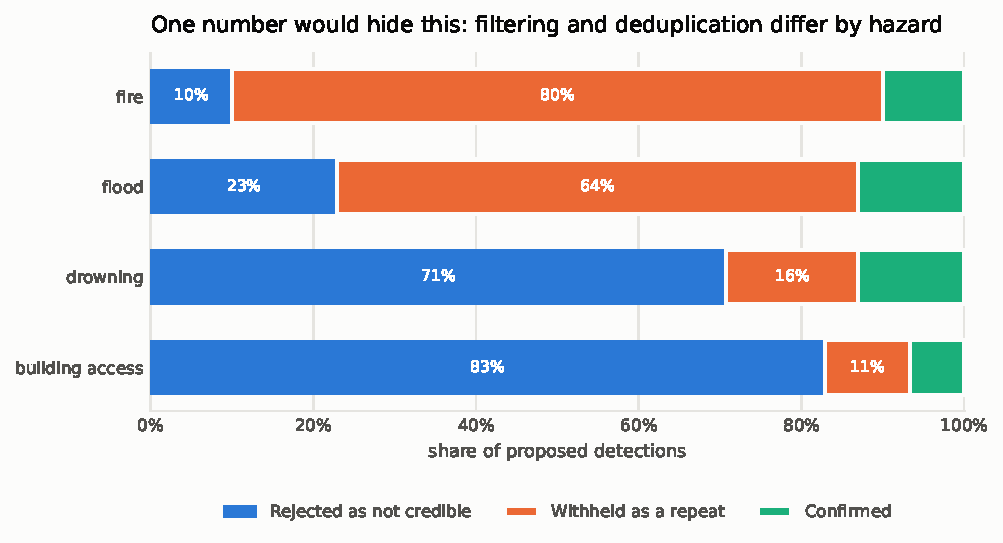
\includegraphics[width=0.9\textwidth]{suppression_split.pdf}
\caption{What the validator does with each hazard's proposals. Fire's headline
suppression is almost entirely the system declining to re-announce one fire it
had already found; building access's is almost entirely filtering. Quoting a
single figure would overstate the false-alarm contribution by a factor of
eight on the fire clip.}
\label{fig:suppression}
\end{figure}

\begin{recorded}{This project has been caught by exactly this before}
During the first ablation, recall appeared to collapse from $0.925$ to $0.125$
and read as the validator destroying the detector. It was cooldown correctly
suppressing repeat alerts about a fire already found — the validator was
locating \emph{more} fires, not fewer. Cooldown was removed from the
evaluation harness for that reason. The runtime pipeline later reintroduced
the same conflation in its live statistics, and now reports the two quantities
separately everywhere they appear, including on the recorded demonstrations
and in the operator interface.
\end{recorded}

\subsubsection{False-alarm reduction}
\label{sec:ablation}

\begin{table}[htbp]
\centering\small
\caption{The validator against the raw detector on
\AblationNegativeSequences{} negative sequences and \AblationFireSequences{}
ignition sequences from HPWREN FIgLib. \measured{} —
\texttt{eval/run\_ablation.py}.}
\label{tab:ablation}
\begin{tabular}{l S[table-format=1.3] S[table-format=2.0] c
                  S[table-format=1.3] S[table-format=1.1]}
\toprule
Configuration & {FAR} & {Reduction \%} & Fires found & {Frame recall}
  & {Min.\ to detect} \\
\midrule
Raw detector, no validator      & \RawFAR       & {—}            & \RawFiresFound/\FiresTotal & \RawFireRecall       & \RawMinutesToDetect \\
Full cascade, persistence $= 3$ & \ValidatedFAR & \FARReduction  & \FiresFound/\FiresTotal    & \ValidatedFireRecall & \MedianMinutesToDetect \\
\bottomrule
\end{tabular}
\end{table}

At persistence 3 the false-alarm rate falls by \FARReduction\,\% and every
fire is still found: \FiresFound{} of \FiresTotal{}, the same as the raw
detector. Sequence-level detection is what matters operationally, and it is
unchanged. A ByteTrack-style second association stage~\citep{zhang2022bytetrack}
— below-floor detections keeping tracks alive without being allowed to alarm
— was also implemented and measured: it changed nothing on either the sparse
ablation or a dense \SI{8}{fps} sequence, because the tracker's miss
tolerance already bridges the gaps it exists to bridge. It ships disabled, as
a documented null result.

Two costs are paid for that, and both sit in \cref{tab:ablation}, not
in a footnote. The median time to first alert rises from
\RawMinutesToDetect{} to \MedianMinutesToDetect{} minutes, and frame-level
recall falls from \RawFireRecall{} to \ValidatedFireRecall{} — the frames
spent accumulating persistence are frames on which the system stays silent
about a fire it can already see. Reporting only the false-alarm reduction
would hide both. A filter that drove false alarms to zero by refusing to alert
at all would score perfectly on the one metric and be useless.

\subsubsection{Comparison with confidence thresholding}
\label{sec:threshold-matched}

\Cref{tab:ablation} compares the cascade against the raw detector \emph{at
the same confidence floor}. That leaves open the objection any careful
reader raises next: forget temporal validation — raise the floor until the
false-alarm rate matches, and see what it costs. Most system papers leave
this control to the reviewer. We ran it, and it partially deflates our own
headline, so it is reported in full.

Sweeping the raw detector's floor over the same cached detections, a floor
of \MatchedFloor{} —
selected \emph{on these very negatives}, so an oracle baseline — reaches the
cascade's false-alarm rate of \CascadeFAR{} while keeping frame recall
\MatchedRecall{} against the cascade's \CascadeRecall{}, all
\MatchedFires{}/\FiresTotal{} fires, and a median time-to-alert of
\MatchedMinutes{} minute against the cascade's \MedianMinutesToDetect. A
floor of \ZeroFARFloor{} drives the false-alarm rate to zero on this set
outright, at frame recall \ZeroFARRecall. \Cref{fig:frontier} shows the
frontier; the cascade's operating point sits below it.

\begin{figure}[htbp]
\centering
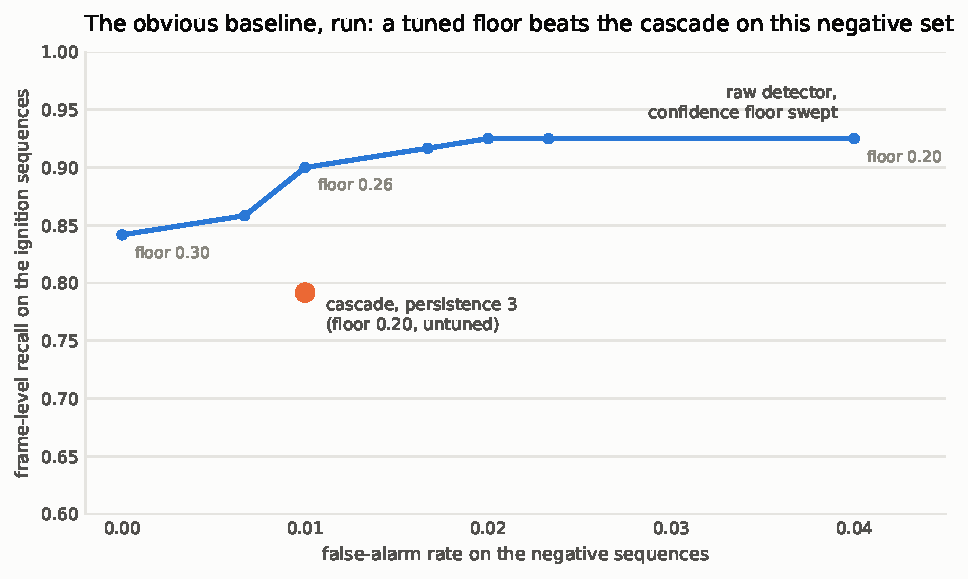
\includegraphics[width=0.9\textwidth]{threshold_frontier.pdf}
\caption{The control experiment
(\texttt{eval/run\_threshold\_matched.py}). Each blue point is the raw
detector at one confidence floor, on identical cached detections; the orange
point is the cascade at persistence 3. On this negative set an oracle-tuned floor
dominates the cascade — the finding this paper reports against itself, and
the reason the claim in \cref{sec:scoped-claim} is scoped the way it is.}
\label{fig:frontier}
\end{figure}

\paragraph{What the control does and does not establish}
\label{sec:scoped-claim}

The control establishes that \textbf{per-frame false-alarm reduction on this
negative set is not the cascade's contribution}: a tuned threshold does it
more cheaply. Three things bound how far that conclusion travels, each a
fact, none a defence:

\begin{itemize}
  \item \textbf{The matched floor is an oracle.} The sweep selects
        $\theta = \MatchedFloor$ using the same 30 sequences it is scored on;
        the cascade runs the detector authors' published default ($0.20$)
        untouched. A deployed threshold must be chosen on some cameras and run
        on others, so the honest comparison is not oracle-against-cascade but
        transferred-threshold-against-cascade. We run that comparison in
        \cref{sec:threshold-transfer-exp}, and it reverses the control's
        verdict.
  \item \textbf{No floor survives the hard negatives.} On the curated
        \texttt{pyro-sdis} negatives (\cref{sec:fire}), raising the floor to
        $0.30$ still leaves a false-alarm rate of $0.648$ while recall is
        already falling — fog and dust are detected \emph{with high
        confidence}. Whether persistence helps there is untested, because no
        temporal hard-negative set exists in any release we know of; building
        one is listed in \cref{sec:outstanding}.
  \item \textbf{Deduplication is not achievable by any threshold.}
        \Cref{tab:decomposition} shows most of what the validator does on
        several hazards is withholding repeats of an event already reported —
        an operational function a per-frame threshold cannot express at all.
\end{itemize}

\paragraph{The transfer experiment: the objection, answered}
\label{sec:threshold-transfer-exp}

The control's central caveat — that its winning floor is an oracle — is
testable, so we test it. The \TransferCameras{} FIgLib negative cameras are
split into two disjoint folds; on one fold the floor is tuned to the target
false-alarm rate, that fixed floor is applied to the \emph{other} fold, and
the result is compared against the cascade running its untuned published
floor on the same held-out cameras (\texttt{eval/run\_threshold\_transfer.py}).
The split is deterministic — cameras sorted and alternated — so no seed has to
be trusted, and both directions are reported.

The oracle does not survive transfer. Tuned to a false-alarm rate of
\TransferTrainFAR{} on one fold (floor \TransferTunedFloor), it drifts to
\TransferTestFAR{} on the cameras it has not seen — more than three times the
target — while the cascade at the published floor holds \TransferCascadeFAR{}
on the same cameras. Tuned the other way (floor \TransferBATunedFloor) it
does hold the false-alarm rate on transfer, but only by \emph{losing a fire}:
recall \TransferBARecall{} against the cascade's \TransferBACascadeRecall.
Averaged over both directions the transferred threshold sits at
\TransferMeanThresholdFAR{} against the cascade's \TransferMeanCascadeFAR.

This reverses the control of \cref{sec:threshold-matched}. A confidence floor
beats the cascade only with oracular access to the negatives it will face; a
floor chosen the way a deployment must choose it either lets false alarms
drift up or sacrifices a detection, whereas the cascade's persistence — being
a property of the tracks, not of any camera's confidence calibration — holds
both false-alarm rate and recall across cameras it has never seen. The
camera-independence of persistence, asserted by an earlier draft, is here a
measured advantage.

The honest statement of the validator's value is therefore this, and it is
now supported by the experiment above rather than by assertion: \emph{a
single untuned mechanism that holds its false-alarm rate and its recall
across unseen cameras where a tuned threshold holds at most one of the two,
provides deduplication no threshold can express, and transfers across hazards
by configuration} — at a measured cost in latency (\cref{sec:latency}) that
is predictable in closed form.
Where a deployment can tune a floor on representative negatives and does not
need deduplication, thresholding alone is the better choice, and this paper
says so.

\subsubsection{Latency cost}
\label{sec:latency}

The latency is not an empirical surprise. Persistence requires $N$ associated
sightings before confirming, so for a camera sampling at rate $f$ the
additional delay relative to a single-frame detector is
\begin{equation}
  \mathbb{E}[\Delta t] \;=\; \frac{N - 1}{f},
  \label{eq:latency}
\end{equation}
assuming the track is not missed. HPWREN's FIgLib cameras sample once per
minute, so at $N = 3$ \cref{eq:latency} predicts exactly
$(3-1)/1 = \SI{2}{\minute}$ of extra delay. The measured medians are
\RawMinutesToDetect{} minutes raw and \MedianMinutesToDetect{} validated, a
difference of \AddedMinutesToDetect{} minutes — the predicted value. The
identity matters more than the agreement: it says the latency cost is a
property of the \emph{camera's sampling rate}, not of the method, so the same
cascade on a camera sampling at \SI{1}{\hertz} costs two seconds. A deployment
choosing $N$ is choosing a point on \cref{eq:latency}, and can be told what it
will cost before any data is collected.

\subsubsection{Cross-hazard transfer}

PyroNear's published training manifest shows that they already perform
sequential confirmation for wildfire, with a grid search over a minimum frame
count. Temporal confirmation for fire is therefore not novel, and we say so.
The claim VIGÍA makes is narrower and still defensible: \emph{one} validator,
configured rather than specialised, working across hazards whose detectors
were built by different people, on different data, for phenomena with
different physics.

\begin{table}[htbp]
\centering\small
\caption{The same validator on two hazards with different physics: a wildfire
plume develops over tens of minutes and is nearly static between frames; a
collision resolves in under a second with objects moving fast across the
frame. The only difference between the two runs is a configuration object.
\measured{} — \texttt{eval/run\_multihazard.py}.}
\label{tab:transfer}
\begin{tabular}{l l S[table-format=3.0] S[table-format=3.0]
                  S[table-format=2.0] S[table-format=2.1]}
\toprule
Hazard & Source & {Frames} & {Raw det.} & {Confirmed} & {Suppression \%} \\
\midrule
Wildfire smoke  & FIgLib, 1 frame/min & \FireFrames    & \FireRawDetections    & \FireConfirmedEvents    & \FireSuppression \\
Road incidents  & Dashcam, 2 fps      & \TrafficFrames & \TrafficRawDetections & \TrafficConfirmedEvents & \TrafficSuppression \\
\bottomrule
\end{tabular}
\end{table}

\subsubsection{Scope of the evidence}
\label{sec:evidence-reach}

The scope of what has and has not been measured deserves an explicit
statement, because the two are easy to conflate. Three distinct kinds of
false-alarm evidence appear in this paper, on different numbers of hazards:

\begin{enumerate}
  \item \textbf{Per-frame detector false-alarm rate}, measured on curated or
        natural negatives, is reported for \emph{three} hazards: fire
        (\FireImageFAR{} on \FireNegatives{} negatives, \cref{sec:fire}),
        people in water (\SwimmerImageFAR, \cref{sec:piw}) and building
        access (\BuildingImageFAR, \cref{sec:building}). This establishes
        that the false-alarm problem the paper motivates is real beyond the
        one detector used for the headline.
  \item \textbf{The temporal validator's false-alarm \emph{reduction}} — the
        cascade against the raw detector on negative sequences, with the
        transfer control — is demonstrated on \emph{one} hazard, fire,
        because it is the only hazard for which negative temporal sequences
        exist in released form. The flood trend detector's false-alarm
        behaviour is measured separately, on stable water with realistic
        segmentation noise (\cref{sec:ph-calibration}), which is a second
        hazard's false-alarm measurement by a different mechanism.
  \item \textbf{Configuration-only transfer} of the cascade across hazards
        with different physics is shown in \cref{tab:transfer}, but that
        table measures suppression, not accuracy against held-out labels.
\end{enumerate}

The honest consequence is that the central causal claim — \emph{temporal
validation reduces the false-alarm rate} — is evidenced directly on fire and
by mechanism-analogue on flood, and that extending it to a second detector
with negative sequences is the single most valuable experiment this work has
not been able to run (\cref{sec:outstanding}). The paper's title says
multi-hazard because the \emph{system} spans four hazards and the validator
transfers to them by configuration; it does not claim the reduction is
independently proven on all four.

\begin{recorded}{Enforced, not merely asserted}
\texttt{tests/test\_validator.py} contains
\texttt{test\_validator\_contains\_no\_hazard\_specific\_code}, which parses
the validator's source with Python's AST module and fails the build if any
comparison against a specific hazard appears. A future contributor fixing a
wildfire bug with a hazard-specific branch cannot silently invalidate the
central claim of this document. The suite passes 9 of 9.
\end{recorded}

\section{Consolidated results}
\label{sec:results}

Every figure VIGÍA has measured to date, in one place. Figures published by
third parties are listed separately in \cref{tab:reported} and are never
combined with ours.

\begin{table}[htbp]
\centering\small
\caption{Measured by us. Every value traces to the results file named in the
last column.}
\label{tab:measured}
\begin{tabularx}{\textwidth}{l L S[table-format=1.4] l}
\toprule
Hazard & Metric & {Value} & Harness \\
\midrule
Fire   & Box precision                          & \FireBoxPrecision  & \texttt{run\_image\_eval} \\
Fire   & Box recall                             & \FireBoxRecall     & \texttt{run\_image\_eval} \\
Fire   & Image-level FAR, \FireNegatives{} negatives & \FireImageFAR & \texttt{run\_image\_eval} \\
Fire   & FAR, no validator                      & \RawFAR            & \texttt{run\_ablation} \\
Fire   & FAR, validator at $N=3$                & \ValidatedFAR      & \texttt{run\_ablation} \\
\addlinespace
Flood  & Water $\iou$, ATLANTIS test            & \FloodWaterIoU     & \texttt{run\_flood\_eval} \\
Flood  & $F_1$, ATLANTIS test                   & \FloodFOne         & \texttt{run\_flood\_eval} \\
Flood  & Water $\iou$, aerial, flooded subset   & \AerialFloodedIoU  & \texttt{train\_flood\_aerial} \\
\addlinespace
People in water & Box $F_1$                     & \SwimmerFOne       & \texttt{run\_person\_in\_water\_eval} \\
People in water & Image-level FAR               & \SwimmerImageFAR   & \texttt{run\_person\_in\_water\_eval} \\
\addlinespace
Building access & Civilian box recall           & \BuildingBoxRecall & \texttt{run\_building\_access\_eval} \\
Building access & Civilian box $F_1$            & \BuildingBoxFOne   & \texttt{run\_building\_access\_eval} \\
\addlinespace
Scene routing   & Held-out accuracy             & \RouterAccuracy    & \texttt{train\_scene\_router} \\
\bottomrule
\end{tabularx}
\end{table}

\begin{table}[htbp]
\centering\small
\caption{Quantities that are not detector accuracy: what the validator does,
what the gate saves, and what the system costs to run. \measured{} on the
reference machine (MacBook Pro M4 Pro, \SI{48}{\gigabyte}), \textsc{reference}
backend.}
\label{tab:system}
\begin{tabularx}{\textwidth}{L l l}
\toprule
Quantity & Value & Source \\
\midrule
False-alarm reduction, validator at $N = 3$   & \FARReduction\,\%   & \cref{tab:ablation} \\
Ignition sequences still detected             & \FiresFound{}/\FiresTotal{} & \cref{tab:ablation} \\
Median time to first alert, raw               & \RawMinutesToDetect\,min & \cref{tab:ablation} \\
Median time to first alert, validated         & \MedianMinutesToDetect\,min & \cref{tab:ablation} \\
Added latency, predicted and observed         & \AddedMinutesToDetect\,min & \cref{eq:latency} \\
Frame-level recall, raw then validated        & \RawFireRecall\ / \ValidatedFireRecall & \cref{tab:ablation} \\
Threshold-matched control: oracle floor       & \MatchedFloor{} reaches FAR \CascadeFAR & \cref{sec:threshold-matched} \\
\quad its recall / latency vs the cascade's   & \MatchedRecall{}\,/\,\MatchedMinutes\,min vs \CascadeRecall{}\,/\,\MedianMinutesToDetect\,min & \cref{fig:frontier} \\
Colour prior: measured and removed            & recall \ColourBaselineRecall{} $\to$ \ColourStrictRecall{} for FAR \ColourBaselineFAR{} $\to$ \ColourStrictFAR & \cref{sec:removed-levels} \\
Suppression, total across four clips          & \SuppressionTotal\,\%      & \cref{eq:decomposition} \\
\quad of which filtering                      & \SuppressionFiltered\,\%   & \cref{tab:decomposition} \\
\quad of which deduplication                  & \SuppressionDeduplicated\,\% & \cref{tab:decomposition} \\
Gate reduction, demonstration registry        & \GateReduction\,\%  & \cref{eq:gate-saving} \\
\quad detector invocations per frame          & \GateGated{} of \GateUngated{} & \cref{eq:gate-saving} \\
Inference latency, \textsc{reference}         & \textasciitilde\SI{60}{\milli\second} & \cref{sec:backends} \\
Inference latency, \textsc{fast}              & \textasciitilde\SI{34}{\milli\second} & \cref{sec:backends} \\
Validator behavioural tests                   & 9/9 passing         & \texttt{tests/test\_validator.py} \\
Registry tests                                & 22/22 passing       & \texttt{tests/test\_registry.py} \\
Flood level tests                             & 13/13 passing       & \texttt{tests/test\_flood\_level.py} \\
\bottomrule
\end{tabularx}
\end{table}

\begin{table}[htbp]
\centering\small
\caption{\reported{}. Published by the people who built each component, listed
here for completeness and never combined with our figures. Where a
model card publishes nothing, that is stated, not filled in.}
\label{tab:reported}
\begin{tabularx}{\textwidth}{l L l}
\toprule
Component & Metric & Value \\
\midrule
PyroNear fire detector    & precision / recall / mAP     & not published \\
PyroNear2025 benchmark    & cross-dataset $F_1$          & \textasciitilde70\,\% \\
RF-DETR SeaDronesSee      & mAP@50, five classes         & \SwimmerAuthorMAP \\
RF-DETR SeaDronesSee      & per-class AP, swimmer        & \SwimmerAuthorAP \\
YOLOv8-DRN (DRespNeT)     & mAP@50, 28 classes, 27\,FPS  & 92.7\,\% \\
Road-incident YOLO11x     & mAP@50                       & 0.826 \\
Road-incident YOLO11x     & accident-class recall        & 0.855 \\
Reference multi-task system & fire FAR 52\,\% $\to$ 4\,\% at 96\,\% sensitivity & \citep{multitasksystem} \\
\bottomrule
\end{tabularx}
\end{table}


\section{Discussion}
\label{sec:discussion}

\subsection{Evaluation commitments}

\begin{itemize}
  \item \textbf{Cross-dataset evaluation.} Domain shift is the most likely
        cause of real-world failure; a random split of the training set
        flatters a model and predicts nothing about deployment.
  \item \textbf{Report the gap.} In-domain and out-of-domain figures appear
        side by side.
  \item \textbf{Event-level evaluation on sequences}, not frame-level on
        stills. The validator only demonstrates value over time.
  \item \textbf{$F_2$ rather than $F_1$ as the headline}, for the reason given
        in \cref{eq:fbeta-ratio}.
  \item \textbf{Never quote a figure we did not measure.} Published
        third-party numbers appear only in clearly attributed rows.
  \item \textbf{Every proportion carries its interval} (\cref{sec:intervals}).
\end{itemize}

\begin{recorded}{A trap we walked into and documented}
Our first false-alarm measurement on ignition sequences gave 0.8\,\%, against
71\,\% on curated hard negatives with the same model and threshold. The
difference is negative-set difficulty: frames shortly before a fire are
usually clear skies, whereas curated negatives are cloud, fog and dust chosen
to confuse. Had we published the 0.8\,\% figure as evidence the validator
works, any reviewer inspecting the negative set would have dismantled the
claim. Every false-alarm figure in this document names the negative set it
came from.
\end{recorded}

\subsection{Execution backends}
\label{sec:backends}

Two backends exist and are not interchangeable. \textsc{reference} runs the
as-published dynamic-shape graph on the CPU provider and is deterministic;
every figure in this document comes from it. \textsc{fast} runs a static-shape
variant on Apple's CoreML provider and is 1.7--1.9$\times$ faster
(\SI{34}{\milli\second} against \SI{60}{\milli\second} at \SI{1024}{\pixel}).

\textsc{fast} is not bit-identical. Across 100 validation frames the detection
count matched on 100 of 100 and boxes agreed to within \SI{0.41}{\pixel}, but
confidences drift by up to $0.012$ because the Neural Engine computes at lower
precision. At the $0.20$ operating point that drift changed no metric; at
$0.10$ and $0.30$ it moved box precision and recall by about one percentage
point by flipping a single detection across the threshold. \textsc{fast} is
therefore used for anything a person watches, and \textsc{reference} for
anything reported.

\begin{recorded}{A parity check that checked nothing}
The ONNX export parity check originally traced the model on random noise. A
trained detector finds nothing in random noise, so the check compared zero
detections against zero detections and passed unconditionally. It now traces a
real frame and reports \textsc{unverified} if that frame yields no detections,
instead of passing quietly.
\end{recorded}

\subsection{Findings}
\label{sec:findings}

Distilled from the measurements, phrased for reuse beyond this system:

\begin{enumerate}
  \item \textbf{Report suppression as two numbers or not at all.} Filtering
        and deduplication differ by a factor of eight between our hazards
        (\cref{tab:decomposition}); one figure conflates a false-alarm claim
        with alert housekeeping.
  \item \textbf{Run the threshold-matched control \emph{and} the transfer
        experiment before claiming alarm reduction.} On negatives it had seen,
        an oracle threshold beat our cascade; across unseen cameras that same
        threshold either let false alarms drift up or lost a detection, while
        the untuned cascade held both. The oracle result alone would have
        misled in either direction; both controls cost an afternoon on cached
        detections.
  \item \textbf{Persistence has a price list:}
        $\mathbb{E}[\Delta t] = (N-1)/f$. The latency cost of temporal
        confirmation is a property of the camera's sampling rate, computable
        before any data is collected.
  \item \textbf{Pooled metrics flatter minority-critical classes.} Selecting
        the aerial flood model on pooled IoU would have chosen a model
        better at recognising dry ground (\cref{sec:pooling}); stratify on
        the case the system exists for.
  \item \textbf{Appearance priors fail where the confuser shares the
        property} — fog is as grey as smoke — and geometric priors can
        invert safety on the severe tail (the worst floods are the largest).
        Measure each level of a life-safety cascade on the negatives it will
        actually face, and be willing to delete.
  \item \textbf{Image-level metrics can hide a dead detector.} A label-shift
        bug survived image-level evaluation at precision $0.83$ and was
        exposed only at box level, at recall $0.002$
        (\cref{sec:twolevels}). Evaluate at both levels, always.
  \item \textbf{Interval or it didn't happen.} At $n = 12$ images, a recall
        of $1.000$ means $[0.757, 1.000]$ (\cref{tab:intervals}); reporting
        the interval is the difference between a measurement and an
        anecdote.
\end{enumerate}

We would argue the transferable contribution is the practice: every
proportion carrying the interval its sample supports, stratified metrics
where pooling flatters, suppression decomposed into the claim it supports
and the housekeeping it is not, controls run against one's own headline, and
twelve retracted claims documented in place. None of this required novel
architecture. All of it changed what the paper was allowed to say.

\subsection{Limitations and outstanding work}
\label{sec:outstanding}

Listed in the order it would be tackled. The first three are shortages of
available material rather than defects in the system.

\begin{enumerate}
  \item \textbf{No temporal hard-negative set exists.} Tuned thresholding
        suffices on easy negatives (\cref{sec:threshold-matched}); no
        threshold survives the curated hard stills; whether persistence
        survives them is untestable without hard negatives that are also
        sequences — fog rolling over a ridge, filmed. Assembling one from
        HPWREN's archive is the single most valuable experiment this project
        has not run.
  \item \textbf{Building access rests on \BuildingTestImages{} held-out
        images.} Strong on that split (civilian box recall
        \BuildingBoxRecall, interval \BuildingCivilianRecallCI{} over
        instances), but twelve positive images cannot make the image-level
        figures precise (\cref{tab:intervals}), and the released data cannot
        be widened. It needs a different post-disaster aerial dataset with
        people annotated.
  \item \textbf{No urban flood footage.} The flood demonstration uses a
        public-domain gauge camera on a creek. The 2024 Valencia DANA is the
        event this system is motivated by, and no footage of a flooded
        street is yet available to it under a licence permitting publication.
  \item \textbf{The road-incident detector has no standalone measurement}
        against held-out labels; it remains the validator's generality
        experiment only.
  \item \textbf{The gauge correlation is one event on one camera}
        ($r = +0.50$, \cref{sec:gage}); it should be repeated across many
        USGS cameras and events before the trend claim is leaned on.
  \item \textbf{The aerial flood segmenter has no held-out split}
        (\cref{tab:flood-aerial}); FloodNet's withheld masks make this
        unfixable from the public release.
  \item \textbf{Night operation.} Fire and flood are evaluated in daylight
        only; the flood segmenter mislabels infrared frames and the fetch
        pipeline excludes them by envelope. Disasters do not keep daylight
        hours — the Valencia flooding peaked in the evening — so an
        infrared-domain evaluation, likely fine-tuned on the USGS cameras'
        own night frames, is required before any claim extends past dusk.
\end{enumerate}


\section{Conclusions}
\label{sec:conclusion}

This paper set out to make published hazard detectors usable on the cameras
cities already operate, and to measure honestly what a shared temporal
validation layer contributes toward that goal. The conclusions the
measurements support are stated below in their final, qualified form.

The system stands: five detectors from four independent sources run behind
one declarative gate with enforced viewpoint envelopes, one temporal
validator confirmed to contain no hazard-specific branch, a privacy boundary
with no biometric code path, and an AGPL-free runtime of four packages —
each property held by a build-failing guard, not a promise. The
validator's value, after the controls of \cref{sec:threshold-matched}, is
scoped to what the measurements support: it reaches an oracle-tuned
threshold's false-alarm rate \emph{without} access to the negative
distribution, it deduplicates alerts as no per-frame threshold can, and it
transfers across hazards by configuration — at a closed-form latency cost
(\cref{eq:latency}) and a measured recall cost that thresholding, where it
suffices, does not pay. Two cascade levels that failed their measurements
were removed, not kept (\cref{sec:removed-levels}).
\paragraph{Data and code availability.} Every figure in this paper is
generated from committed measurement files by the build described in
the released repository, including the training and
evaluation scripts that reproduce each number, accompanies this paper.

\paragraph{Acknowledgments.} This work runs on other people's science, named
throughout: the PyroNear association and the
French SDIS; HPWREN at UC San Diego, whose imagery appears here under its
attribution requirement; the U.S. Geological Survey's streamgage camera
network; the authors of ATLANTIS, FloodNet, SeaDronesSee, DRespNeT and
V-FloodNet; and the maintainers of ONNX Runtime, NumPy, OpenCV and
torchvision.


\bibliography{refs}

\end{document}
